% $Id: jfsample.tex,v 19:a118fd22993e 2013/05/24 04:57:55 stanton $
\documentclass[11pt]{article}

% DEFAULT PACKAGE SETUP

\usepackage{setspace,graphicx,epstopdf,amsmath,amsfonts,amssymb,amsthm,versionPO}
\usepackage{marginnote,datetime,enumitem,subfigure,rotating,fancyvrb}
\usepackage{hyperref,float}
\usepackage[longnamesfirst]{natbib}
\usdate
\usepackage{lscape}
\usepackage{amsmath}


% These next lines allow including or excluding different versions of text
% using versionPO.sty

\excludeversion{notes}		% Include notes?
\includeversion{links}          % Turn hyperlinks on?

% Turn off hyperlinking if links is excluded
\iflinks{}{\hypersetup{draft=true}}

% Notes options
\ifnotes{%
\usepackage[margin=1in,paperwidth=10in,right=2.5in]{geometry}%
\usepackage[textwidth=1.4in,shadow,colorinlistoftodos]{todonotes}%
}{%
\usepackage[margin=1in]{geometry}%
\usepackage[disable]{todonotes}%
}

% Allow todonotes inside footnotes without blowing up LaTeX
% Next command works but now notes can overlap. Instead, we'll define 
% a special footnote note command that performs this redefinition.
%\renewcommand{\marginpar}{\marginnote}%

% Save original definition of \marginpar
\let\oldmarginpar\marginpar

% Workaround for todonotes problem with natbib (To Do list title comes out wrong)
\makeatletter\let\chapter\@undefined\makeatother % Undefine \chapter for todonotes

% Define note commands
\newcommand{\smalltodo}[2][] {\todo[caption={#2}, size=\scriptsize, fancyline, #1] {\begin{spacing}{.5}#2\end{spacing}}}
\newcommand{\rhs}[2][]{\smalltodo[color=green!30,#1]{{\bf RS:} #2}}
\newcommand{\rhsnolist}[2][]{\smalltodo[nolist,color=green!30,#1]{{\bf RS:} #2}}
\newcommand{\rhsfn}[2][]{%  To be used in footnotes (and in floats)
\renewcommand{\marginpar}{\marginnote}%
\smalltodo[color=green!30,#1]{{\bf RS:} #2}%
\renewcommand{\marginpar}{\oldmarginpar}}
%\newcommand{\textnote}[1]{\ifnotes{{\noindent\color{red}#1}}{}}
\newcommand{\textnote}[1]{\ifnotes{{\colorbox{yellow}{{\color{red}#1}}}}{}}

% Command to start a new page, starting on odd-numbered page if twoside option 
% is selected above
\newcommand{\clearRHS}{\clearpage\thispagestyle{empty}\cleardoublepage\thispagestyle{plain}}

% Number paragraphs and subparagraphs and include them in TOC
\setcounter{tocdepth}{2}

% JF-specific includes:

\usepackage{indentfirst} % Indent first sentence of a new section.
\usepackage{endnotes}    % Use endnotes instead of footnotes
%\usepackage{jf}          % JF-specific formatting of sections, etc.
\usepackage[labelfont=bf,labelsep=period]{caption}   % Format figure captions
\captionsetup[table]{labelsep=none}

% Define theorem-like commands and a few random function names.
\newtheorem{condition}{CONDITION}
\newtheorem{corollary}{COROLLARY}
\newtheorem{proposition}{PROPOSITION}
\newtheorem{obs}{OBSERVATION}
\newcommand{\argmax}{\mathop{\rm arg\,max}}
\newcommand{\sign}{\mathop{\rm sign}}
\newcommand{\defeq}{\stackrel{\rm def}{=}}

\begin{document}

\setlist{noitemsep}  % Reduce space between list items (itemize, enumerate, etc.)
\onehalfspacing      % Use 1.5 spacing
% Use endnotes instead of footnotes - redefine \footnote command
%\renewcommand{\footnote}{\endnote}  % Endnotes instead of footnotes

\author{Maria Kurakina  \thanks{\rm Haas
      School of Business, University of California, Berkeley; E-mail: maria\_kurakina@berkeley.edu; 
      Tel: 510-926-0289. I am indebted to my advisors, David Sraer, Ulrike Malmendier, Lee Fleming, and Dmitry Livdan, for their support and guidance. Special thanks to Coleman Fung Institute for Engineering Leadership and Guan-Cheng Li for providing the access to patent application database. I would also like to thank Benjamin Balsmeier, Gustavo Manso, Amir Kermani, Yuriy Gorodnichenko, Hoai-Luu Nguyen, Carlos Avenacio-Leon, Tristan Fitzgerald, Christopher Lako, Troup Howard, Dayin Zhang, Nicholas Sander, Marius Guenzel as well as numerous seminar participants at the Haas School of Business and Economics Department at UC Berkeley for their valuable comments and suggestions.}}

\title{\Large \bf The Dark Side of Patents: \\ Effects of Strategic Patenting on Firms and their Peers}

\date{UC Berkeley - Haas School of Business \\ October 2019}              % No date for final submission

% Create title page with no page number

\maketitle
\thispagestyle{empty}

\bigskip

\centerline{\href{https://drive.google.com/open?id=16sPbbTuUI3Qpzp1b1G8gfT1VrnZ90d62}{Click here for most recent version}}
\centerline{\bf ABSTRACT}
%\begin{doublespace}  % Double-space the abstract and don't indent it
  \noindent 
  Prior literature on innovation focuses predominantly on the “bright side” of patents: By increasing a firm’s total factor productivity and through positive spillovers patenting activity contributes to the aggregate economic growth. This paper provides evidence that firms can benefit even from patents of low productive value, by instead focusing on the main purpose of patents: capturing market share and defending monopolistic profits of firms. This is achieved by deterring entry in the same product market. I introduce the new way of defining such “strategic” patents by combining data on stock market based measures of economic value of patents and citation-weighted patent counts. This new measure is consistent with the previously used alternative ways of defining strategic patents, while being superior in terms of market coverage and computational accessibility. Using data on patent applications, I find that strategic patenting by firms leads to an increase in market concentration, while productive patents make markets more competitive. This observation is supported by the negative effect that strategic patenting has on number of firms operating in a product market. At the same time, strategic patents have a smaller but still positive effect on the total factor productivity of firms, while having a significant positive effect on profit growth. There is no positive spillover to other firms operating in the same product market. For the closest competitors, I observe a reduction in both profit and total factor productivity growth following strategic patenting. 
  
%\end{doublespace}

\medskip


\clearpage

\section{Introduction} \label{sec:Intro}

 In the recent years the question about the benefits of patenting to the firm and the market as a whole has no longer become obvious. The earlier literature focused heavily on emphasizing the positive aspects of patents as an embodiment of innovative activity of the firm, leading to sales growth, job creation and increase in firms' total factor productivity. But this "bright side" of patents is just one side of the coin, as firms can benefit through issuing the patent not from the straightforward productivity gains a patented innovation can bring to the company, but from the harm a new patent can do for the firm's competitors in the same product market. 

The idea of these so called "strategic patents" is widely theoretical, but their existence is yet to be demonstrated empirically in a general market setting. In this paper I will shed some light on what are strategic patents, how do they shape the industry environment, what firms tend to engage in this type of patenting, and whether the strategic patents are ex ante identifiable by the market.


I introduce the definition of strategic patent combining the observation of \color{blue} Acigit et al (2013) \color{black} on the non-linear nature of the relationship between the economic value of the patent and its scientific value (measured by the number of forward citations) and \color{blue} Kogan et al (2017)\color{black} stock market based measure of private value of innovation. Strategic patents exhibit negative relationship between forward citations and economic value of the patent as opposed to the positive relationship conventionally attributed to productive patenting activity -- more technologically valuable patents bring higher value to the innovating firm as well as high positive spillovers to the market (reflectd in higher forward citations). Strategic patents are usually done as continuation patents to the highly valuable productive patents received by the firm earlier. Another name that can be given to such patent type is "defensive" as the main purpose of the patent is to protect the exclusive rights granted by the productive patent and thus defend the firm against possible entrants in this product market, which can deprive it of the monopolistic profit. 

This paper introduces a new measure of defining strategic patents, consistent with previous literature observations on characteristics attributed to this type of patents and their effect on innovative market activity. Using this definition, the following hypothesis about the nature of strategic patents are tested in this paper. First, as a patent aimed at defending the firm's market share, I expect the decrease in market competition following strategic patent issue. Secondly, compared to regular productive patents, exhibiting the positive relationship between the patent economic value and forward citations, strategic patents should lead to the lower growth in firm's total factor productivity. Highly cited high valued patents are such due to their radical nature as innovation thus increasing the firm's labor productivity and creating positive spillovers for potential market entrants and existing competitors. On the other hand, strategic patents derive its high value not from the patent's contribution to firm's technological improvement (be that through new product line introduction or development of a more cost effective production process), but from protection it offers to the previously granted productive patents, thus not adding to total factor productivity increase. A third hypothesis tested in this paper is the negative effect on the patenting firm peers' outcomes (reduction in growth of profit, output and total factor productivity) following a strategic patent. This effect is especially strong for strategic patents issued by technological leaders within the product market. At the same time this mechanism behind strategic patenting leads to the boost of profits of patenting firm generated by the recent break-through discoveries in the field compared to the effect of similar productive patents not supported by the follow up strategic one. The results are robust to controlling for competitors innovative activity. 


%FIX LITERATURE REVIEW
This paper contributes to the following strands of research. First and foremost, his paper extends the analysis of the effect of patent issue on firm performance outcomes from the patenting firm itself to its peers using the whole universe of market industries. The standard literature on the impact of innovation (and patenting activity as its representation) focused mostly on how it affected the firms' own performance, firm's stock market price and market value \color{blue}(Pakes 1986, Hall, Jaffe, Trajtenberg 2001, Kline, Petkova, Williams, Zidar 2017, Farre-Mensa, Hegde, Ljungqvist 2015, Balasubramanian, Sivadasan 2011, Kogan, Pappanikolau, Seru and Stoffman 2017)\color{black}. Of the papers examining the effect on rival firms it is worth pointing out \color{blue}Austin (1993)\color{black}, which only looks at a small sample of the biotechnology industry in early 1990s,and papers by \color{blue} Megna and Klock (1993), Jaffe, Trajtenberg, and Henderson (1993), Cockburn and Henderson (1994)\color{black}, examining the R\&D spillovers effect again only on a subsample of industries. These studies conclude that firms are benefiting from the patents of rival firms, though there is still some evidence that patent rights can impose costs on rival firms -- the idea which is further developed and is the main focus of this paper. 

Secondly this is the first paper to empirically illustrate the difference in effect of strategic patent on patenting firm market structure, performance of the patentee, and its closest product market peers. Previous literature on strategic use of patents (\color{blue} Abrams, Akcigit, Popadak (2013), Farrell and Shapiro (2008) and Noel and Schankerman (2013), Hall and Ziedonis (2001), Ziedonis (2004), Hegde, Mowery, and Graham (2009), Galasso and Schankerman (2010), Cockburn and MacGarvie (2011), and Von Graevenitz, Wagner, and Harho (2013)\color{black}) examine either the theoretical implication of strategic patenting, or on the empirical side they look at its effect on the subsequent patenting activity by the firm and within the patent technology class, mostly with a focus on a specific technological industry. This paper introduces a novel approach of identifying the strategic patent based on both the data on patent forward citations as well as market stock return based measure of patent value introduced in \color{blue} Kogan et al (2017)\color{black}. This method allows me to test the implications of issuance of strategic patent by the firm for the whole sample of patenting public firms.   


The rest of the paper is organized the following. Section 2 describes the data and empirical setting, including the methodology of constructing economic value of patent used in patent classification into strategic and productive. Sections 3 outlines the empirical strategy, while Section 4 present the main results on the strategic patent effect on market concentration, firms' TFP and profit growth and effect on its peers' outcomes. Section 5 discusses alternative interpretations of results and presents robustness checks. Section 6 concludes.        

\section{Empirical Setting and Data} \label{sec:Data}

The approach of identifying strategic patents among the firm's patent portfolio relies on finding an appropriate measure of economic value of the patent. In this section I discuss the methodology of estimating return based patent value introduced in \color{blue} Kogan, Pappanikolau, Seru and Stoffman (2017)\color{black}. After describing the data used in this paper I illustrate that using this measure of patent value one can consistently identify strategic patents from productive by testing the already established in  the literature observations about strategic patent behavior (i.e. strategic patents being more likely continuation and divisional patents, more prevalent in recent years, and leading to decrease in innovative activity by competitors within the product market).       

\subsection{Motivation for Patenting}

Patents play an important role in firm value creation process. Owning a U.S. patent gives firm the exclusive right of making and selling its innovation within the country. Patent ownership can be used by firms to enter a new profitable market attracting extra revenues thus positively affecting its balance sheet, increasing the profit margin and leading to overall increase the firm's share prices and valuation. This direct sources of income derived from patent ownership range from patent licensing and ownership transfer to entering the litigation process with the purpose of obtaining the damages for patent infringement \color{blue}(Miele (2000))\color{black}.  

Apart from the direct profit firm extracts from its patent ownership, it can also derive an indirect benefits namely from the defensive nature of patents that leads to the increase in the patenting firm market share. Thus, patents can be used as means of deterrence of competitors from operating or entering patentee's product market. Even a threat of potential patent infringement suit can lead to the delay of competitor's entry into the new market, which can have negative effect on firm's growth and overall presence within the industry as well as the number of patents filed within the same product market following strategic patent.

While most valuable patents generate both direct (revenue increasing -- \textit{productive} value) and indirect (entrance deterring -- \textit{strategic} value) benefit to its owners, recent studies have shown the resurgence of patents of predominantly strategic value: Patents whose sole purpose is to prevent subsequent entry into the given product market and thus protecting the profits generated by related productive patent issued to this firm -- mostly continuation applications, focused on a different aspect of the same technology, or divisional applications, focusing on a particular invention mentioned in the original patent. 

An example of continuation strategic patent is "slide-to-unlock" patent by Apple from October, 2012 \footnote{Examples from IP Asset Maximizer blog from January 24, 2014 "Strategic Patenting Part: Why So Few Patents Create Real Value" by Jackie Hutter, see \url{http://ipassetmaximizerblog.com/strategic-patenting-part-1-why-so-few-patents-create-business-value/}} . This is a third patent in the series of "slide-to-unlock" patents issue by the firm. The initial patents specified the "predefined path" of the movement on screen to unlock the device, which was an easy obstacle for competitors to overcome and avoid patent infringement suits. The newly issued patent on the other hand covers any uninterrupted movement on touch-sensitive display which leads to unlocking the device. Hence, one can classify this patent as strategic as: 1) it was being extremely effective in preventing other firms in the industry from using this design without licensing in their devises thus making Apply products superior and more desirable in the eyes of the customers, therefore protecting the monopolistic profit the firm was deriving from previous
productive patents; 2) it was not contributing more to the technological advancement since it is not a breakthrough invention -- the novelty of this particular invention, a.k.a slide-to-unlock mechanism, has already been manifested in the previous two patents, which is reflected in the low number of forward citations this patent received compared to its predecessors.

This example illustrates the distinctive characteristic of strategic patents, which is the high economic value of such patent despite its low scientific contribution as estimated based on number of forward citations. This observation implies that the previously established positive relationship between patent value and forward citations (i.e. papers as \color{blue}Harthoff et al (1999), Hall et al (2005), Nicholas et al (2008) \color{black} find statistically significant positive effect of patent citations on excess return) is no longer valid for high valued patents. 


\subsection{Measure of Economic Value of the Patent}

For computing the empirical measure of \textit{economic value} of patent I follow the approach introduced by \color{blue}Kogan et al (2017) \color{black} based on the firm’s stock market movement as a response to the patent application announcement. 
Economic value of the patent (or, as the authors call it, \textit{private} value $\xi_j$) is constructed as the product of market capitalization $M_j$ of the firm at $t = - 1$, where $t$ is the date of filing the patent by the firm, and an estimate of stock return related to the patent issue $\mathbb{E}[{\upsilon_j|r_j}]$. This product is weighted by the number of patents issued by this firm during the same day $N_j$, and adjusted by unconditional probability of a patent application being successful $\bar{\pi}$ \color{blue}(Carley, Hegde, and Marco (2015) \color{black} estimate it being 56\%): 
\begin{equation} \label{eq:kogan}
\xi_j = (1-\bar{\pi})^{-1} \frac{1}{N_j} \mathbb{E}[{\upsilon_j|r_j}] M_j
\end{equation}


I construct economic value of innovation for each patent of each firm in my sample using this approach.I use the filing date of the patent as opposed to granting date as in  \color{blue}Kogan et al (2017)  \color{black} in
order to be able to control for the value of the patent for application that were eventually rejected by
the patent examiner office. To ensure that stock fluctuations only reflect the patent announcement related events, following \color{blue}Kogan et al (2017) \color{black} I decompose the stock return into patent specific (value of the patent) and patent unrelated components, and assume that the private value of the patent follows normal distribution truncated at zero (thus suggesting that to the patenting firm a patent has necessarily a positive value). 

As for the\textit{ scientific value} of the patent, which is an estimated the total knowledge contribution
of the patent, I use the number of patent's forward citations (this measure is available for granted
patents only). This variable suffers from truncation problem: that is, more recent patents tend to
have less forward citations by construction due to an increasing number of missing observations
stemming from filed but not yet granted patent applications citing this particular innovation  \color{blue}(Hall,
Jaffe, Trajtenberg (2001))\color{black}. To alleviate this issue in my measure I will control for the time period
over which the forward citations were measure. The availability of data on citations up to the year
2018 allows me to compute forward citations over the period of 5 years after granting of the patent.
Figure 1 illustrates the distribution of patent forward citations over the years of patent filing using
both raw and truncated (over the next five years only) measure. As evident from the graph, the
distribution of raw citations is heavily skewed to the right, which is no longer present for measure
of scientific value based on a five-year window.


Using the new economic value of patent based on firm's stock market movement as a response to patent application I confirm that using this measure one can replicate the inverted U-shape relationship between the private measure of patent and its scientific value as in \color{blue}Akcigit et al (2013) \color{black} by regressing number of patent forward citations on economic value fo the patent and patent value squared using the subsample of granted patents. Results are presented in \autoref{tab:Table1}.

All specifications control for year of filing, examiner art unit and firm fixed effect. Standard
errors are clustered at examiner art unit by filing year level. Both measures of patent economic and
scientific value are normalized to unit standard deviation for ease of result interpretation. Using the
new measure for patent value we still get the positive relationship between the value of patent and
forward citations at all sample winsorization levels, while inclusion of the quadratic term, which is
highly significant, does not leads to the deterioration of overall fit.

Hence, based on the observation of non-linear relationship between economic value and forward
citations for high valued patents the following analysis conducted in this paper will focus on the
differences in the effect strategic patents have on patentee and its competitors in comparison to
productive (scientific) patents. The patent is defined as strategic (scientific) if it falls into the top
50\% of the distribution of the private economic value of the patent as measure by eq.\eqref{eq:kogan}, but
bottom (top) 50\% of distribution of its scientific value \color{blue}(Balsmeier, Kurakina, Stiebale, Fleming
(2018))\color{black}.


\subsection{Data and Sample Selection}



To estimate the effect strategic patents have on industry and individual firms operating within
the market, I construct the dataset combining information on individual patent applications, firm
stock market return, balance sheet information and total factor productivity, and product market
participants list.

The data on patent application number, invention U.S. classification, filing date, publication
date, issue date, and patent number comes from the public-use administrative data provided by
United States Patent and Trademark Office (USPTO). I use the sample of patent applications filed
after November 29, 2000 and published by 31 December 2013, as this is the starting point when
USPTO started providing information on rejected patent applications in addition to only patented
ones. The information on rejected applications is used as control group to compare the effect of
the impact of granting of the strategic vs scientific patent on firm's and its peers performance. I
merge this dataset with administrative data from USPTO Patent Application Information Retrieval
(PAIR) to get information on patent examiner identification as well as examiner art unit (similar
to  \color{blue} Klein et al (2018)\color{black}). The information on application assignee name and patent citations for
granted patents is extracted from Google Patents and is provided by Coleman Fung Institute for
Engineering Leadership.

Each patent application is matched to the respective corporations that filed for the patent based
on the probabilistic record linkage as in \color{blue}Wasi, Flaaen (2014), Hall et al (2001) \color{black} using name of the
patent assignee and name of the firm in CRSP/Compustat Merged database. Additionally, I use
\color{blue}Hall, Jaffe, Trajtenberg (2001) \color{black}patent technology categories classification, which divides all patent
applications into 6 broad technology groups based on patent U.S. technology class and subclass.
The technology classes which were not previously attributed to one of the categories by \color{blue}Hall et al
(2001) \color{black} are I add to one of the categories by hand.

To identify strategic patents from scientific ones, the patent application data is merged with the
information on daily stock return from CRSP dataset. Firm and its competitors profitability and
performance data comes from CRSP/Compustat Merged database. Product market competitors
are defined using Text-based Industry Classification TNIC3 as in \color{blue}Hoberg and Phillips (2010, 2016)\color{black}.
For the analysis I use only the top 50th percentile of closest product market competitors, determined
based on the product description proximity score accompanying the every firm pair in TNIC3. An
average patentee in any given year has 49.64 closest competitors.

All continuous variables are winsorized at the 5th and 95th percentiles of their distributions.
The financial accounting variables are adjusted for inflation using the CPI from Bureau of Economic
Analysis using 2014 as the base year.

I make the following restrictions for my sample. First, I drop all patent applications that are
not matched based on assignee name, leaving me with a sample of public firms only. Secondly,
I limit the analysis to utility patents only. Third, I focus only on applications filed by a single
assignee to avoid the possible complications related to the joint ownership of the patent. Finally,
I only keep companies that have 5 or more years of pre- and post- filing outcomes to make sure
I have enough observations covering the post-filing and post-granting period for the subsample of
eventually granted patents (patent approval takes on average 22 month or more). These sample
restriction leave me with 102,807 patent applications filed by 1,423 firms, out of which 57.11\% were
granted.

\section{Research Design} \label{sec:Data}
\subsection{Identification} 

For both patenting firm and its peers I run the following regression relating the post-patent
filing outcomes to patent strategic status:
\begin{equation} \label{eq:reg1}
y_{i,t} = \alpha + \beta X_i + \gamma I(PatentGranted_i) + \delta I(StrategicPatent_i)+\epsilon_{i,t}
\end{equation}


where \textit{i} denotes patenting firm or the portfolio of patenting firm peers, \textit{t} is the year of patent filing,
is the effect of patent being granted, $\delta$ is the effect of strategic patent being granted as opposed
to other granted patents, $X_i$ is the vector of firm controls including firm previous year's return
on assets, cash flow, firm's Q, sales volatility and growth, leverage, and TNIC3 based Herfindahl
Index, and $\epsilon_{i,t}$ is noise.

This equation suffers from the potential endogeneity problem, where both the estimates of $\gamma$
 and $\delta$ end up being biased if the status of the patent (rejected or accepted) and its strategic characteristic
 are correlated with unobservable characteristics of later firm outcomes: $\mathbb{E}[ \epsilon_{i,t}|I(PatentGranted_i)] \neq
 0$ and $\mathbb{E}[ \epsilon_{i,t}|I(StrategicPatent_i)] \neq
 0$. For example, at the time of filing the firm might be of the
 higher intrinsic quality, thus being able to both file for a more valuable patent and thus having
 it granted as it is being a novel innovation, and at the same time improve its future performance
\color{blue}(Farre-Mensa et al (2015))\color{black}. Thus, it is possible, that post-filing outcomes are
simultaneously determined with the type of the patent the firm files. To solve this issue, I will
employ the matching technique as in \color{blue}Blackwell et al (2009), Angrist (1998), Card et al (1988), and Sarsons (2017)\color{black}.

\subsection{Matching Procedure}

Use of matching as an empirical tool helps to control for the confounding effect of the pretreatment variables in the data, thus improving the balance between the control and treated groups, making them more similar in terms of covariates distribution. I implement the coarsened-exact match for granted and non-granted patents as well as for strategic and other patents within the matched granted subsample. Using my starting sample of filed applications  described in Section 2.3 consisting of 102,807 distinct observations, I first perform an exact match between granted and non-granted patents on the year of patent application filing and its technological category, and I match coarsely on the size of the patentee and economic value of the application using an average of 25 bins for each variable. I repeat this procedure the second time on a subsample of granted patents only, matching between the strategic and non-strategic granted patents. For both matches I match with replacement of individual patents but only let each patent pair to be matched only once. 

\autoref{tab:matched} Panel A shows the comparison between the economic values of the patent of the control and treatment groups (granted vs non-granted patents and strategic vs all other granted patents). By construction there is no difference between the economic value of the patent between the three groups (non-granted, strategic, other granted patents) at 5\% significance level. At the same time strategic patents exhibit a significantly lower number of forward citations than other patents within the matched sample also by construction as evidence from Panel B. This table illustrates the main goal of this matching procedure, namely first and foremost controlling for economic value of the patent, thus avoiding the case of the effect of strategic patenting on the performance of the patentee being driven purely by higher economic value of the patent for strategic as opposed to scientific and non-granted applications (i.e. in general higher performing patents). 

\autoref{tab:matched_sum} and \autoref{tab:matched_sum_s} present summary statistics for the final samples by type of issued patent, comprised of 8,858 granted -- non-granted pairs, and 4,430 strategic -- non-strategic granted patents. All variables are calculated as firm averages over the five year period before patent issue. Firms issuing strategic patents tend to have lower baseline profit, return on assets, less growth opportunities measured by Tobin's Q, as well as being more financially constraint (lower cash flows and higher leverage). At the same time there is no significant difference between the two samples in terms of sales and total assets (by matching sample constriction -- controlling on firm size), and R\&D costs. 

\section{Results}
\subsection{Strategic Patent Characteristics}

As a starting point for evaluating the causal effect of strategic patenting, I begin with a descriptive analysis of strategic and productive patents. Following the previous studies (\color{blue} Akcigit et al (2013)\color{black}), \autoref{tab:cont_age} illustrates the prevalence of continuation and divisional patents among patents issued for purely strategic reasons thus extending the patent protection covering the previously patented technology. This strategy is less beneficial for scientific (truly productive) patents, as the marginal benefit of extending the patent persecution is lower. Columns (1) and (2) of \autoref{tab:cont_age} illustrate that both for the full and matched samples of granted patents issuing a strategic patent increases the likelihood of the patent being either continuation or division one by 3.37-3.96 percentage points compared to other granted patents. 

In addition, I replicate the analysis of Figure 9 from \color{blue} Akcigit et al (2013)\color{black} examining the growth in the occurrence of strategic patenting though time. \autoref{tab:cont_age} columns (3) and (4) confirm the previous studies' observation of the increase in use of strategic patenting by firms in recent years: there is a decrease in granted patent age, measured relative to patent application filing date, if the patent is strategic.  

\autoref{tab:stifle} shows the effect strategic patenting has on innovative activity withing the same product market. One of the main goals of a strategic patent is to stifle further innovative activity in the field, which thus manifests in lower forward citation. Using the change in the average number of patents applied by the closest firm competitors one, three and five years compared to applications submitted over the same period before the patent application by the focal firm, one can observe the significant decrease in the patents issued following a strategic patent as opposed to productive one: on average competitors file for 3.04 (8.26) less patents three (five) years after a strategic patent than they did three (five) years before. This effect is especially pronounced within product markets with lower product proximity between the firms -- competitors operating within more diverse product markets, as illustrated in \autoref{tab:stifle_prox}. The market product proximity is measure as an TNIC3 industry average firm-by-firm pairwise similarity score from \color{blue}Hoberg, Phillips (2010)\color{black}. One possible interpretation of this result is that strategic patenting prevents competitors from extending their business operations into patentee's product niche, hence keeping the peers at bay within the product market. 

The three results discussed above (prevalence of continuation/divisional patents and younger patents among strategic ones, and their effect on stifling innovation in the product market) confirm that the newly introduced measure of strategic innovation based on stock market response to the patent application and number of forward citations is consistent with the previously described in the literature characteristics attributed to strategic patenting.   
   
   
   \subsection{Strategic Patent Effect on Market Concentration and Firm's Performance}
In the following two subsection I show three main results. I first establish that strategic patenting leads to increase in market concentration, the effect which is more pronounced within more product diverse markets. Then I show the difference in the effect strategic patents have on firm’s total factor productivity and profit growth as opposed to productive patents. Finally, I illustrate the negative consequences strategic patenting has on competitors’ productivity and profitability, which is even stronger if the patentee is a technological leader in the market.

\autoref{tab:result_hhi} shows the results of the estimation of equation \eqref{eq:reg1} on a sample of top performing patent applications only (applications with economic value of the patents falling into top 50\% of the value distribution). The coefficients of interest are $\gamma$, which shows the effect of granting of the productive patent on the outcome, whereas $\gamma+\delta$ shows the impact of the strategic patent issuance. The dependent variable is the outcome averaged over five post-filing years. All specifications control for filing year, firm and examiner art unit fixed effects. Standard errors are clustered at examiner art unit by filing year.

Testing the first hypothesis on the effect of strategic patent on industry concentration, I use Herfindahl-Hirschman Index based on Compustat data on firm’s net sales and \color{blue} Hoberg, Phillips (2010) \color{black} TNIC3 industry classification. 

\begin{equation}
\label{eq:hhi}
	HHI_{jt}=\sum_{i=1}^{F_i} s^2_{ijt}
\end{equation}


\noindent where $ s^2_{ijt}$ is the squared market share of year t firm i in industry j, where market shape is computed as a ratio of firm’s sales to total industry j sales, and $F_j$ is number of firms within the product market. Due to use of TNIC3 classification, HHI is firm specific as each firm has a unique set of competitors in each year. 
The results of the effect of strategic patent on market concentration are presented in columns (1) and (2) of \autoref{tab:result_hhi}. Compared to column (1), column (2) additionally controls for baseline patenting firm level characteristics $X_i$ described in Section 3.1. There is a significant increase in market concentration following strategic patent issue by the patentee, while granting of a productive patent leads to the increase in the competition in the market over the next five years. There results are further reinforced by columns (3) and (4), which shows that strategic patenting decreases the number of competitors. These estimates are consistent with the definition of the purpose of strategic patenting – protection of the market share of the patenting firm and preventing competitors entry into the product market – thus, an increase in average post-strategic patent filing HHI. These results are stronger again within more product diverse industries, as evident from \autoref{tab:result_hhi_prox}. Only for markets with average competitors’ market proximity score lower than the year’s median is the effect of strategic patents on industry concentration is significant and positive (negative for number of industry competing firms). Additional dimension of the effect heterogeneity which is investigated in this paper is the level of technological advancement of the patentee. \autoref{tab:result_hhi_gap} shows the results of the regression (2) on market concentration and number of competitors interacted with the patentee’s relation to technological frontier as introduced in \color{blue}Aghion et al (2005)\color{black}. The firms is defined as a technological “leader” if its technological gap is lower than median value, signaling that the firm is closer to the frontier firm. If the gap is larger than the median year’s median value, then the firm is classified as a “laggard”. The technological gap is defined as:

\begin{equation}
\label{eq:gap}
	Gap_i=(TFP_{F,t}-TFP_{i,t})/ TFP_{F,t}
\end{equation}


\noindent where F (for “frontier”) is the firm with the highest total factor productivity within the industry in year t. 
The effect of strategic patent on market concentration is larger for laggard firms as opposed to leaders. This striking point shows which types of firms benefit from filing strategic patents: laggard firms, not being able to “keep up” and compete successfully with their product market peers through the race of novel innovative ideas tend to resort to defensive measures such as having a strategic patent to protect their market share and profits. 
The second hypothesis which is tested in this paper is on the contribution of strategic patenting to firms total factor productivity. While productive “novel” innovation leads to higher mark-ups and improvement of firms’ productivity, thus positively contributing to aggregate economic growth, patenting for strategic purposes does not have technological advancement as a main goal. On the contrary, they are aimed at supporting and preserving the monopolistic profit generated by the previously productive patents issued by the firm, thus being patents of low scientific value. This gap between the effect of productive vs strategic patents on firms total factor productivity is illustrated in columns (5) and (6) of \autoref{tab:result_hhi}.  I use revenue based total factor productivity as in \color{blue}Imrohoroglu et al (2013)\color{black}, which is the measure of the capital and labor effectiveness free of the effect of measured firm costs. The results show a significant increase in total factor productivity of firms following a productive patent issue. Strategic patent grant on the other hand leads to 79\% lower but still positive effect on total factor productivity as opposed to productive patent, thus confirming the low contribution of strategic patents to the post-filing total factor productivity. 
   
\subsection{Effect on Firm’s and it’s Peers’ Future Growth and Productivity}
I now turn to the question of whether strategic patenting has an effect on firm and its competitors performance. Using the same matched sample of top performing patents, \autoref{tab:firm_gr}  shows the result of estimating equation \eqref{eq:reg2}, where the dependent variable is the growth of firm’s profit, sales and total factor productivity ($Y_{i, t+\tau}$) over the horizon $\tau$ of one to five year in future post patent filing:
\begin{equation}
\label{eq:reg2}
log Y_{i,t+\tau} - log Y_{i,t}  = \alpha + \beta X_i + \gamma I(PatentGranted_i) + \delta I(StrategicPatent_i)+\epsilon_{i,t}
\end{equation}



Results of \autoref{tab:firm_gr} show that productive patent grant has a negative effect on firms’ profit growth in the short run up to two years following the patent announcement. Relative to the productive patents, strategic patents exhibit a long run positive increase in profit growth three years and later after the patent issue, while there is not significant effect of productive patents in the long run. Hence, implementation of novel innovative technologies puts a strain on the profitability of the company as it also generates the positive product market spillovers, thus leading to the increase in market competition (as shown in \autoref{tab:result_hhi}) and dilution of monopolistic profits of the patentee. Panel C shows that the effect on profit growth does not come from sales increase, as there is no effect of either strategic nor productive patent grant on firm sales growth.
In case of total factor productivity growth, Panel C of \autoref{tab:comp_gr} shows no significant contribution of strategic patenting activity, consistent with the hypothesis of low contribution of strategic patent to innovation knowledge pool. All increase in TFP growth comes purely from productive patent issue, especially over the long run – four and more years after the patent application. 

I now turn to the question whether strategic patents have a negative spillover effect on firm’s closest competitors, results of which are presented in \autoref{tab:comp_gr}. All competitors outcome measures as well as controls are measured as the equally weighted average over all patentee’s peers within the industry defined as TNIC3.  The analysis in  \autoref{tab:comp_gr} shows significant but short lived (two years after the patent application) negative effect on the average growth rate of competitors’ profit following strategic patenting, which is followed by the negative long run effect of novel (productive) patents, which manifests itself over four years after the patent. Similar trend is observed for competitors’ sales growth, thus providing support to the idea of market share capture by the patentee through strategic patent issue. 
Panel C of \autoref{tab:comp_gr} examines the relation between the type of innovative activity by the firm (strategic or productive) and closest competitors’ productivity. Compared to the absence of effect of strategic patent issue of firm’s own total factor productivity growth, strategic patenting leads to the decrease in peers’ productivity growth over the first three years after the patent issue, consistent with the observation that strategic patent issue by the focal firm not only does not provide positive knowledge spillovers, but on top of that stifles innovative activity within the product market (as previously shown in  \autoref{tab:stifle}).

Last but not least  \autoref{tab:firm_comp_gr} reports subsample results. The negative effect of strategic patent grant on competitors’ productivity and performance growth is larger for product markets in which the patent is being filed by the industry technological leader. This result may be due to competitors taking a more severe hit in sales and productivity when trying to compete with the market leader that already dominates the market, making the competition even tighter. In addition, profit and sales growth is affected most within the less product diverse markets, where issue of strategic patent cuts their sales and forcing them out of their own product market. Interestingly, the opposite is true for the effect on competitors productivity growth: the coefficient on strategic patent grant is significant and negative within less diverse product markets. One potential explanation is the inability of competitors to extend their operations and innovative activity into the patentee’s product market niche, thus limiting their options for growth while staying within their own product market.

\subsection{Robustness}
In this section I discuss the external validity of my results for the strategic patent filers within my estimation sample. 
One potential alternative source of the result significance can be derived from the simultaneity of the innovative activity among the firms within the same product market. That is, the effect on firm’s and competitors productivity and performance can be driven not by the strategic patent per se, but from the fact that the competitors themselves filed for the patent in that year, thus, as we have seen from \autoref{tab:firm_gr} Panel A (effect on patentee’s profit growth) could dampen the profit growth in the first years after the patent file. To alleviate this concern, I rerun the analysis in \autoref{tab:comp_gr} adding the average number of patents filed by the firm’s competitors within the year of firm’s patent application. In  \autoref{tab:robust_p} one can clearly see that the results are not at all driven by the innovation by competitors themselves. 

Next, I examine robustness of the results controlling for merger and acquisition activity of both the patentee and its peers. 

\color{red}…TBA\color{black}

\section{Conclusion}
In this paper, I introduce a new way of classifying patents based into strategic (purely defensive) and productive (scientific). I show that consistent with previous research strategic patents are more likely to be fall into continuation and divisional category, and confirm the recent resurgence of strategic patenting activity in the economy. Using this new market based measure of categorizing the patents, I estimate the impact of strategic patenting by the firm on market concentration, firm productivity and competitors’ performance and productivity outcomes. I find that compared to truly novel productive patents, increasing the firm product market concentration shown by the significant increase in firm specific Herfindahl-Hirschman Index computed based on TNIC3 industry classification, an observation confirmed by the decrease in number of competitors in the market following the strategic patent grant. In addition, strategic patent grant leads to the increase in firm’s long term profit growth, while having much lower tough still positive impact on the revenue-based total factor productivity of the firm compared to scientific patents. I find evidence of the harmful impact strategic patent has on the closest firm competitors, leading to the significant decrease in average sales and profit growth, as well as decrease in peers’ productivity growth, combined with the drop of innovative activity. 

These results confirm the existence and main purpose of strategic patents in protecting the firm’s market niche and preventing the competitors from entry. This paper provides new evidence on detrimental effect of specific type of patent activity to innovation, and thus through this channel to aggregate economic growth. The estimates presented in the paper suggest that patentees have a higher incentive to file such defensive patents than productive ones, thus compromising the product market structure and leading to the increase in monopolization at the expense of technological progress. 

The implications of these results are especially important to be considered during the patent examination process. The patent examination office should enforce stricter rules on patent selection process to allow only truly “innovative” patents be allowed to be patented, thus preventing the firms to exploiting the patent system from undergoing aggressive campaigns on getting strategic patents. The main limitation of this paper’s analysis is that it is yet impossible to establish ex-ante the type of patent the firm has filed for. Thus, this paper should be viewed as the first step into the direction of identify the impact of strategic patenting on the market and its participants \cite{NBERw21959}. 

\pagebreak
\bibliographystyle{plain}
\nocite{*}
\bibliography{references}


\pagebreak
\section{Figures and Tables}
\begin{table}[ht!]\centering
	\def\sym#1{\ifmmode^{#1}\else\(^{#1}\)\fi}
	\captionsetup{singlelinecheck=off}
	\caption[.]{\textbf{. Effect of Private Value of Innovation on Forward Citations.} This table shows the results of regression of number of forward citations on economic value of the patent and value of the patent squared. The economic value of the patent is constructed using equation \eqref{eq:kogan}; the number of forward citations is measured over the period of five years after the patent grant. The table uses the data on full sample of granted patent, taking into account the sample restriction criteria described in Section 2.3. The economic value of the patent is normalized to unit standard deviation and winsorized at the top and bottom 1, 5 or 10\% level for columns (1) and (2), columns (3) and (4), and columns (5) and (6) respectively. The patent value is scaled to unit standard deviation. All specifications control for filing year, examiner art unit and firm fixed effect. Standard errors are clustered at examiner art unit by year of filing. Standard errors are reported in parenthesis. Levels of significance: *10\%, **5\%, and ***1\%.     
			}
	\label{tab:Table1}
	\vspace*{0.2in}		
	{\scriptsize
		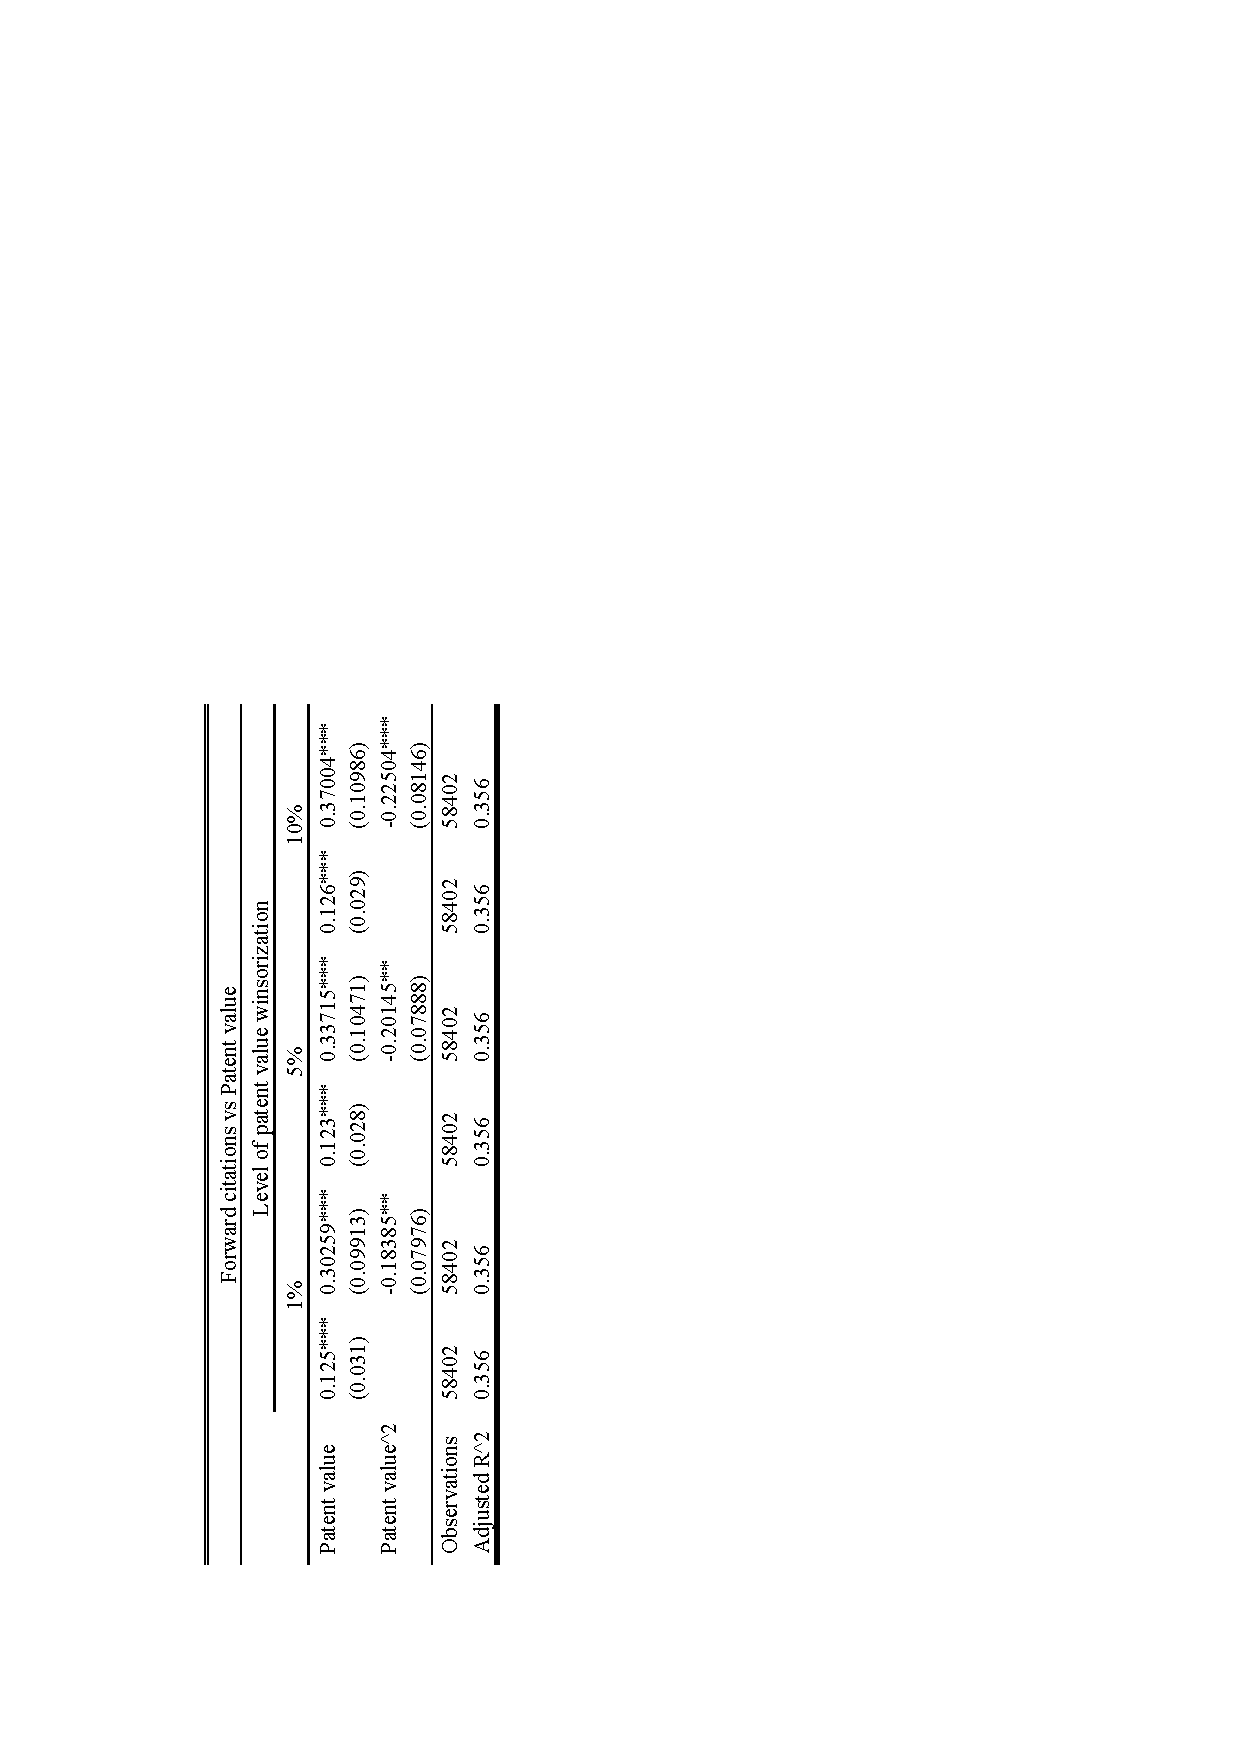
\includegraphics[angle =270,trim = 90 65 300 40, clip]{latex_tables/table_1.pdf}
	}
\end{table}	

\pagebreak
\begin{table}[ht!]\centering
	\def\sym#1{\ifmmode^{#1}\else\(^{#1}\)\fi}
	
	\captionsetup{singlelinecheck=off}
	\caption[.]{\textbf{. Matched Sample for Granted vs Non-Granted, and Strategic vs Productive Patents.} This table shows summary statistics for economic value of the patent (eq.\eqref{eq:kogan}) and its scientific value (forward citations) for the matched sample of granted and non-granted patent applications, and strategic vs scientific within the subsample of granted patents only. The samples are matched exactly on year of patent filing and patent category, and it is matched coarsely on the economic value of the patent and firm's baseline sales outcome (averaged over five pre-filing years). Patents are classified into strategic and productive based on what part of private economic value and forward citations distribution the patent falls: top 50\% of economic and bottom 50\% of forward citation distribution for strategic (top\%50 and top\%50 for productive). The economic value of the patent and forward citations are normalized to unit standard deviation and winsorized at 5\% using annual breakpoints.   
	}
	\label{tab:matched}
	\vspace*{0.2in}		
	{\scriptsize
		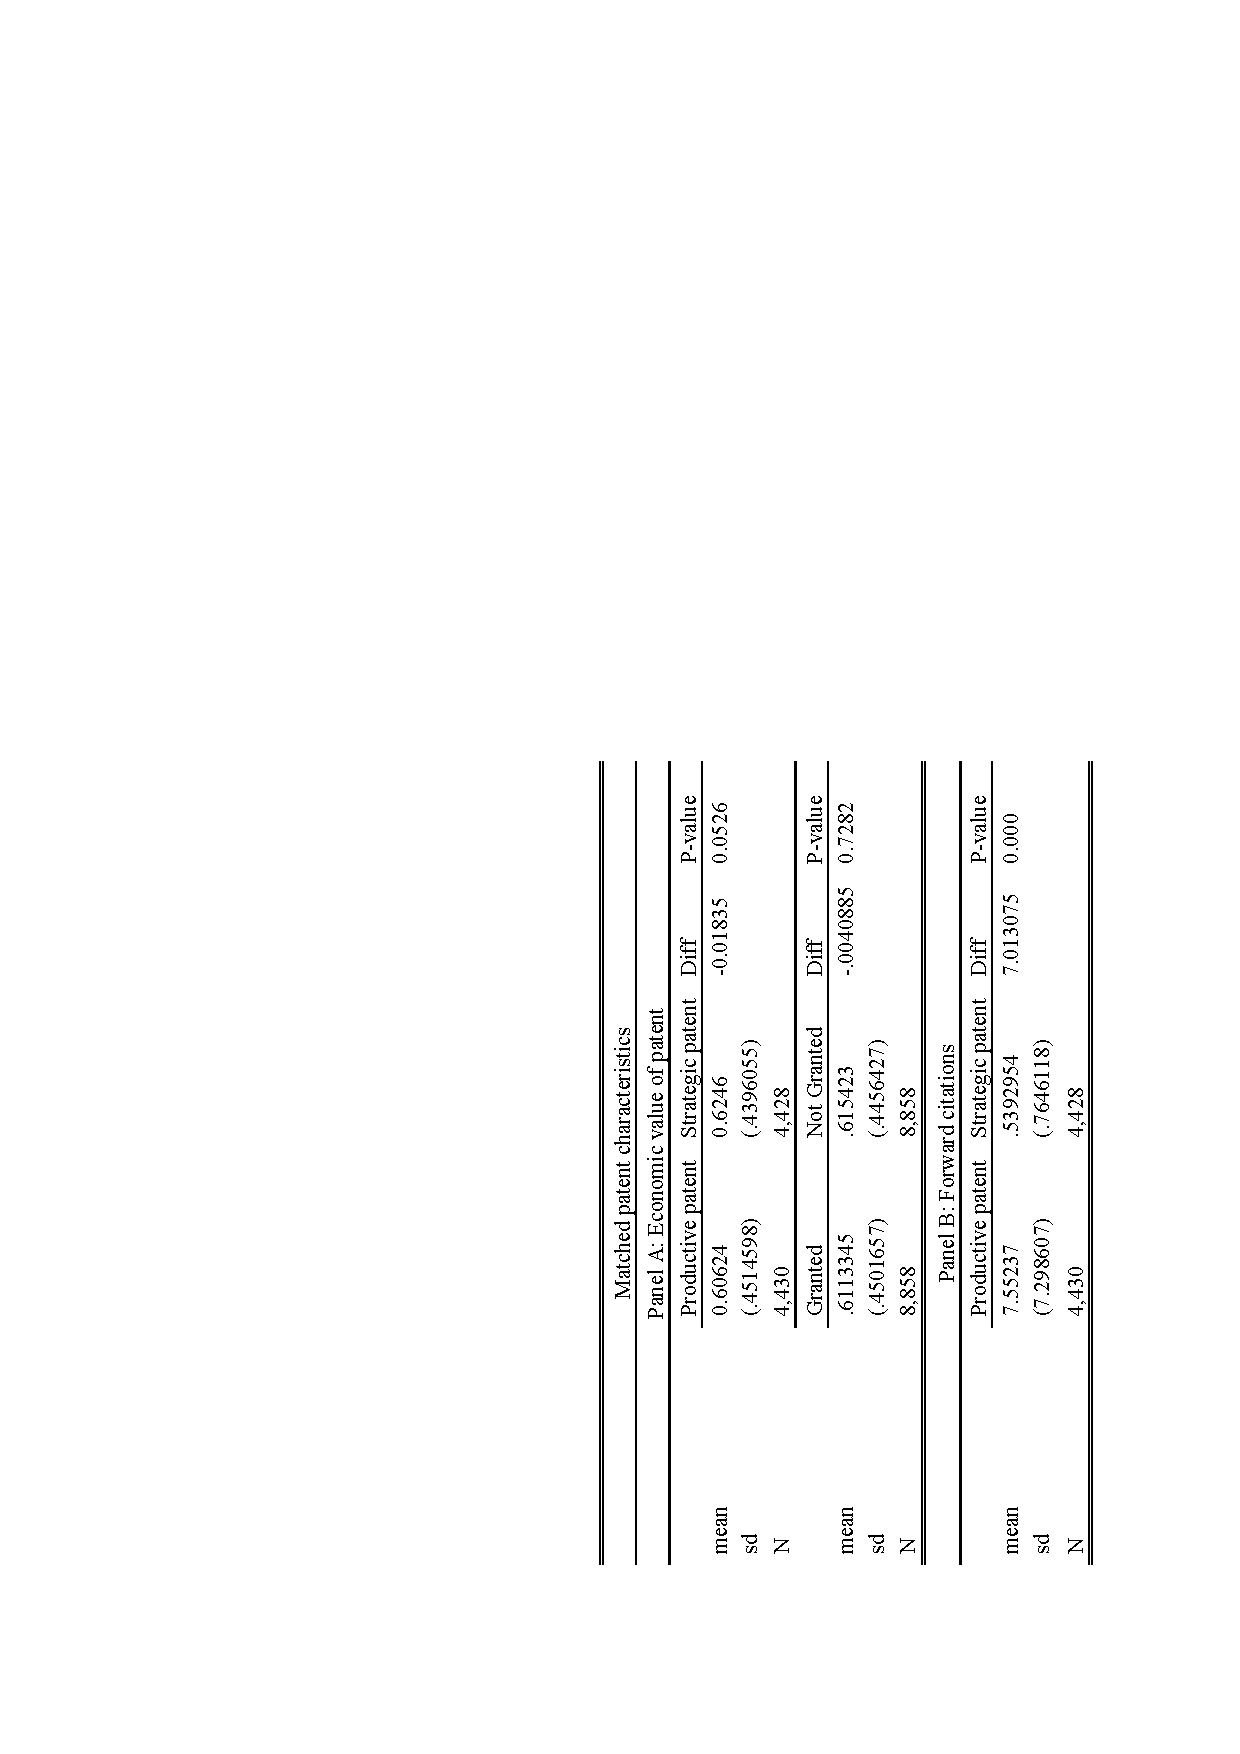
\includegraphics[angle =270,trim = 270 65 40 40, clip]{latex_tables/table_2.pdf}
	}
\end{table}	

\newpage
\begin{landscape}
	\begin{table}[ht!]\centering
		\def\sym#1{\ifmmode^{#1}\else\(^{#1}\)\fi}
		
		\captionsetup{singlelinecheck=off}
		\caption[.]{\textbf{. Summary Statistics: Matched Sample.} The table reports the summary statistics for the full matched sample. The sample is matched exactly on year of patent filing and patent category, and it is matched coarsely on the economic value of the patent and firm's baseline sales outcome (averaged over five pre-filing years). Profit is sales minus cogs, divided by lagged total assets. R\&D is the ratio of firm's research and development expenditures to lagged total assets. Assets is firm's total assets. ROA is the ratio of income before extraordinary items to assets. Tobin's Q is the ratio of the sum of total assets and the difference between market and book value of total common equity, to total assets. Leverage is the sum of long term debt and debt in current liabilities divided by total assets. HHI is Herfindahl-Hirschman Index of industry defined by TNIC3 classification (\color{blue}Hoberg, Phillips (2010)\color{black}). Sales, cogs, CAPX, and cash flows are defined as a ratio to firm's total assets. Each baseline variable is measured as an average over five pre-filing years. All monetary values are expressed in real 2014 dollars. All variables are winsorized at 5\% using annual breakpoints.   
			  
		}
		\label{tab:matched_sum}
		\vspace*{0.2in}		
		{\scriptsize
			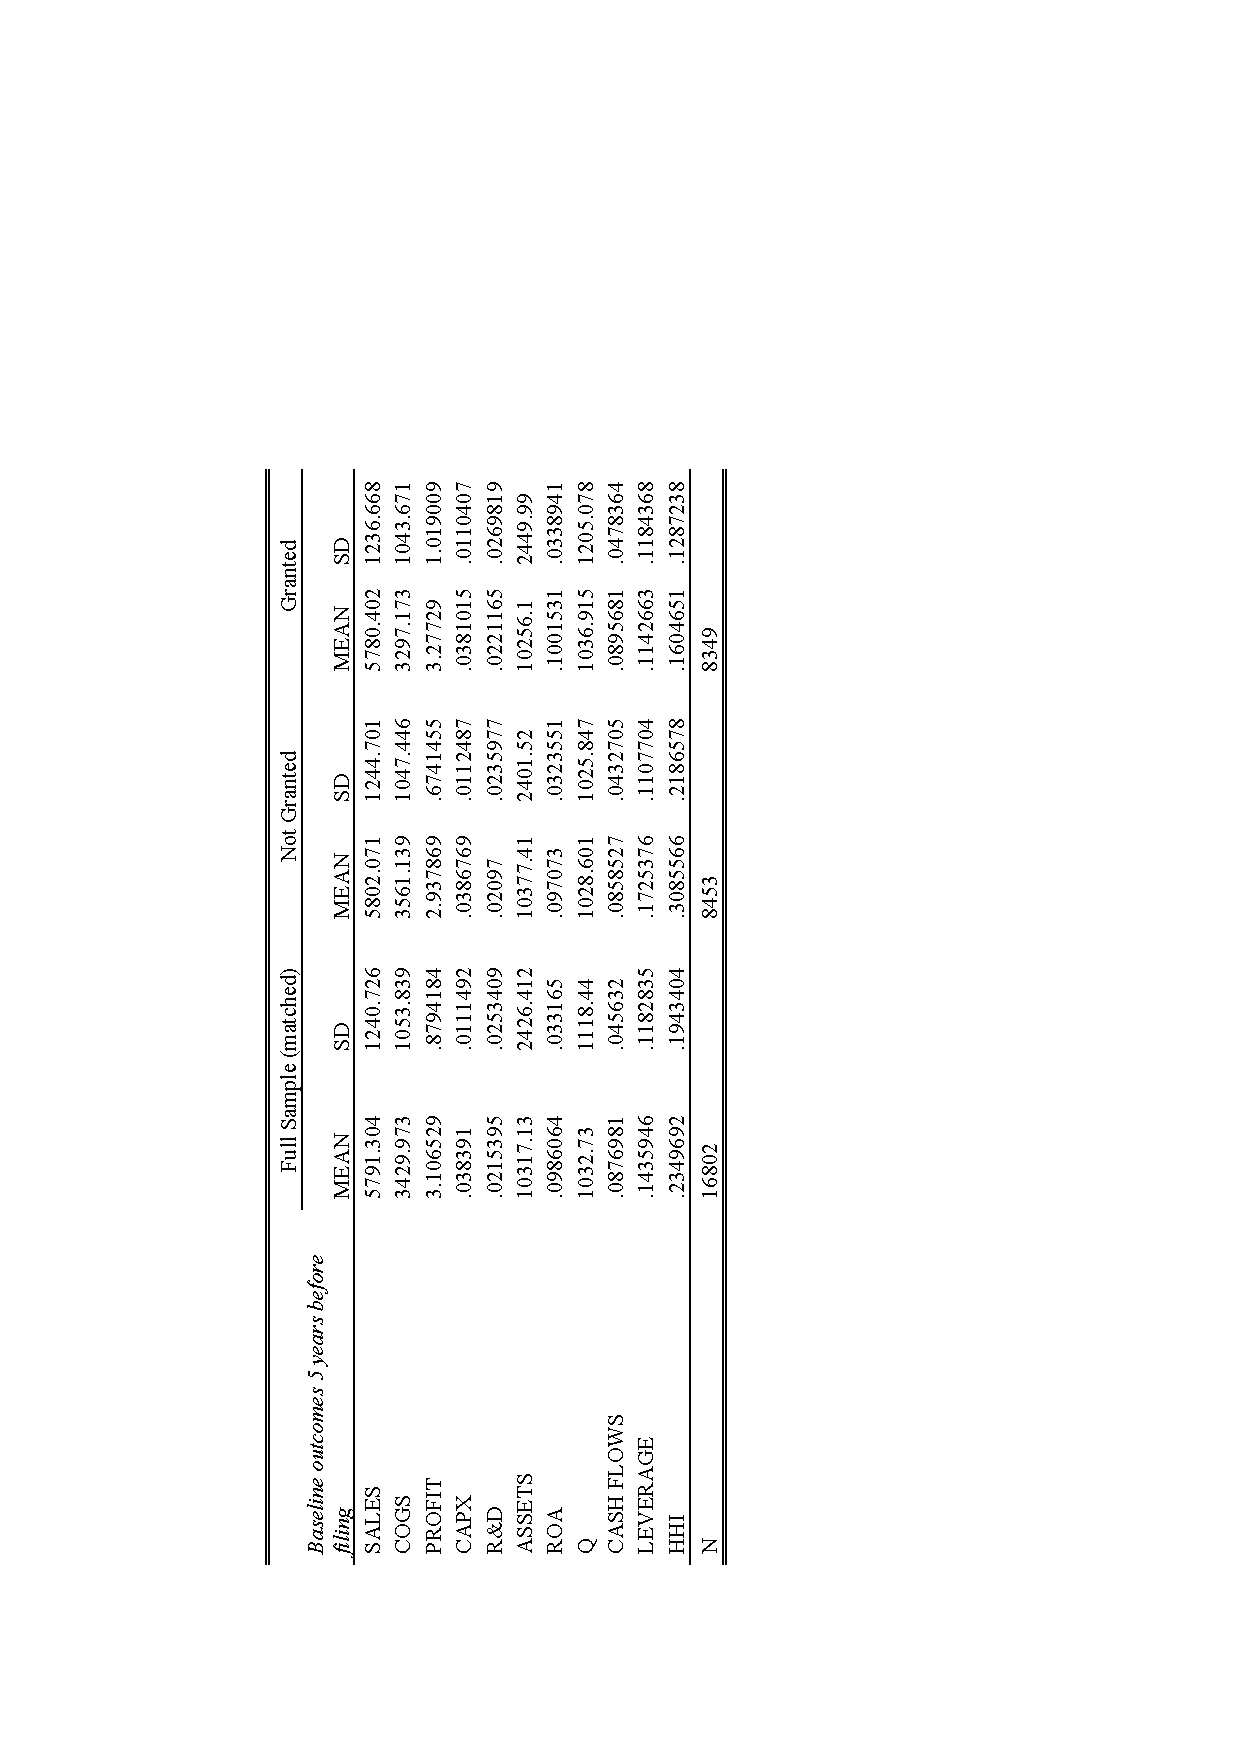
\includegraphics[angle =270,trim = 90 65 40 40, clip]{latex_tables/table_3.pdf}
		}
	\end{table}	
\end{landscape}


\newpage
\begin{table}[ht!]\centering
	\def\sym#1{\ifmmode^{#1}\else\(^{#1}\)\fi}
	
	\captionsetup{singlelinecheck=off}
	\caption[.]{\textbf{. Summary Statistics: Matched Sample -- Strategic vs Productive Patents.} The table reports the summary statistics for subsample of strategic and productive patent subsamples.  The sample is matched exactly on year of patent filing and patent category, and it is matched coarsely on the economic value of the patent and firm's baseline sales outcome (averaged over five pre-filing years). The patent is classified as strategic (productive) if it falls into the top 50\% of the distribution of the private economic value of the patent as measure by eq.\eqref{eq:kogan}, but
		bottom (top) 50\% of distribution of its scientific value (measured by forward citations).  Profit is sales minus cogs, divided by lagged total assets. R\&D is the ratio of firm's research and development expenditures to lagged total assets. Assets is firm's total assets. ROA is the ratio of income before extraordinary items to assets. Tobin's Q is the ratio of the sum of total assets and the difference between market and book value of total common equity, to total assets. Leverage is the sum of long term debt and debt in current liabilities divided by total assets. HHI is Herfindahl-Hirschman Index of industry defined by TNIC3 classification (\color{blue}Hoberg, Phillips (2010)\color{black}). Sales, cogs, CAPX, and cash flows are defined as a ratio to firm's total assets. Each baseline variable is measured as an average over five pre-filing years. All monetary values are expressed in real 2014 dollars. All variables are winsorized at 5\% using annual breakpoints.}
	\label{tab:matched_sum_s}
	\vspace*{0.2in}		
	{\scriptsize
		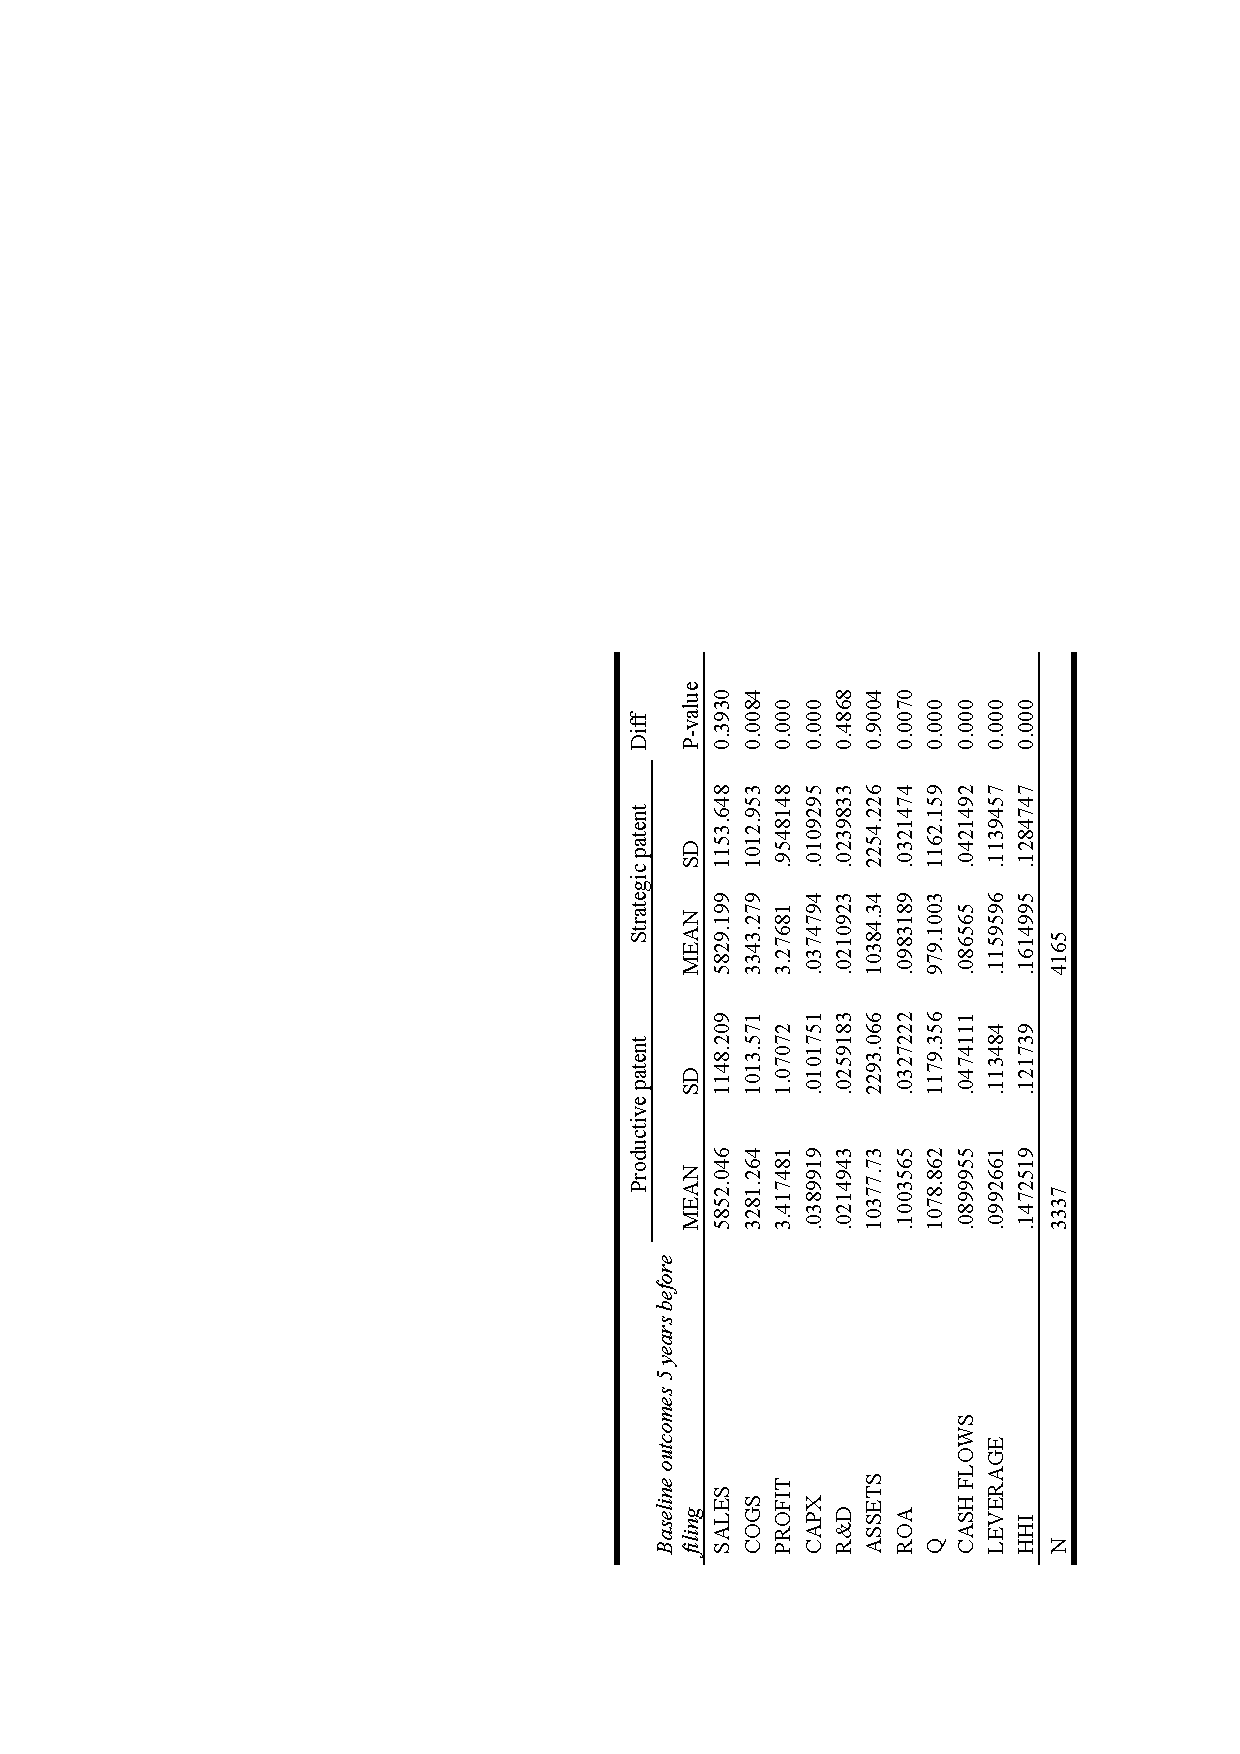
\includegraphics[angle =270,trim = 280 65 70 40, clip]{latex_tables/table_4.pdf}
	}
\end{table}	

\newpage
\begin{table}[ht!]\centering
	\def\sym#1{\ifmmode^{#1}\else\(^{#1}\)\fi}
	
	\captionsetup{singlelinecheck=off}
	\caption[.]{\textbf{. Strategic Patent Characteristics.} Table reports the results of regression of an indicator of patent strategic status on probability of the patent being a continuation (USPTO PAIR: CON -- continuation, CIP -- continuation in part) or divisional patent (USPTO PAIR: DIV), and on patent age, measured relative to the date of patent filing date. The results are estimated on the sample of top performing patents in the full (non-matched sample) and matched sample. Patent applications are classified as top performing if at the date of patent filing the economic value of the patent is higher than the year's median. All specifications control for filing year, examiner art unit and firm fixed effect. Standard errors are clustered at examiner art unit by year of filing. Standard errors are reported in parenthesis. Levels of significance: *10\%, **5\%, and ***1\%.    
	}
	\label{tab:cont_age}
	\vspace*{0.2in}		
	{\scriptsize
		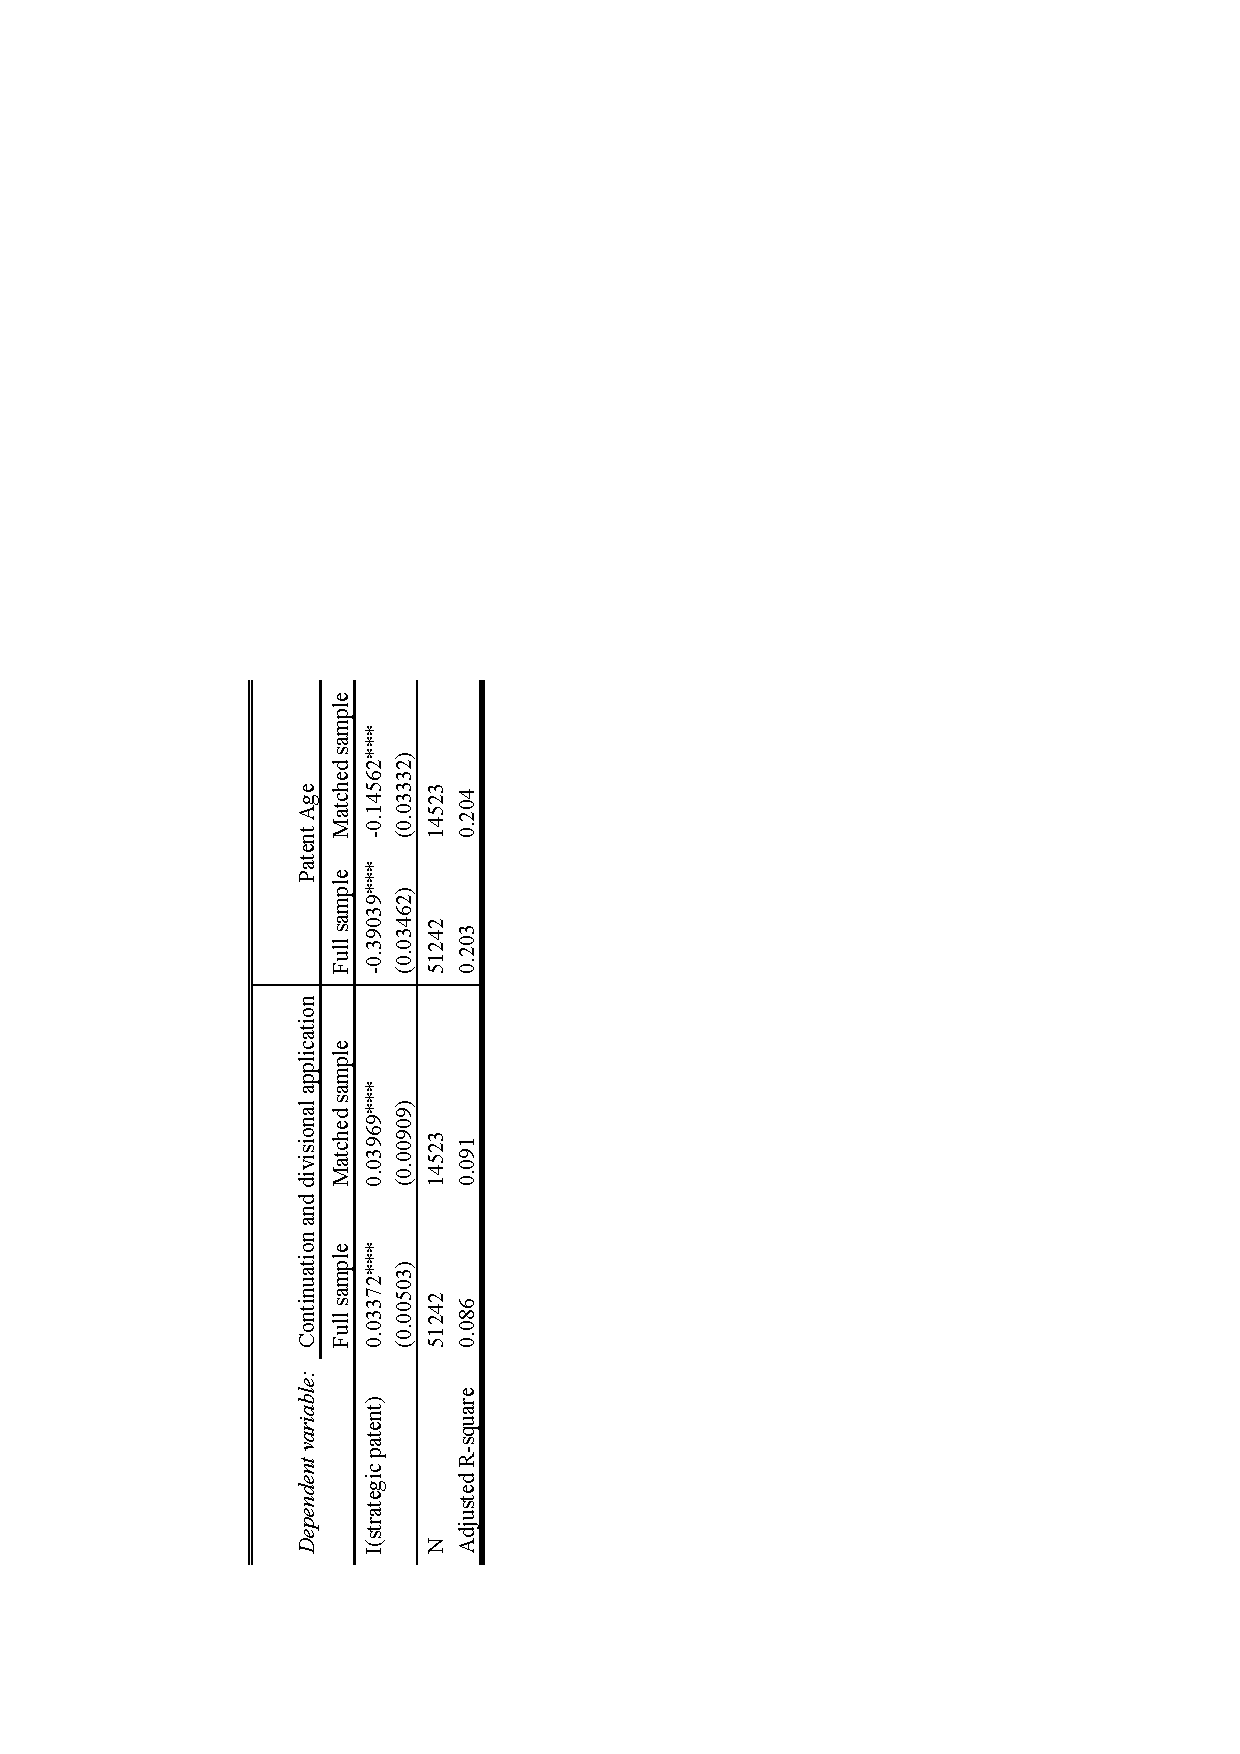
\includegraphics[angle =270,trim = 110 65 350 40, clip]{latex_tables/table_5.pdf}
	}
\end{table}	

\newpage
\begin{table}[ht!]\centering
	\def\sym#1{\ifmmode^{#1}\else\(^{#1}\)\fi}
	
	\captionsetup{singlelinecheck=off}
	\caption[.]{\textbf{. Strategic Patent Effect on Innovation by Competitors.} Table reports the results of regression of an indicator of patent strategic status on the change in number of patents filed by the competitors within the same product market defined by TNIC3. Columns (1) through (3) use the difference between the total number of patents issued by competitors one, three and five years after and one, three and five years before the filing of the patent by focal firm respectively. The results are estimated on the sample of top performing patents within the matched sample. Patent applications are classified as top performing if at the date of patent filing the economic value of the patent is higher than the year's median. All specifications control for filing year, examiner art unit and firm fixed effect. Standard errors are clustered at examiner art unit by year of filing. Standard errors are reported in parenthesis. Levels of significance: *10\%, **5\%, and ***1\%.
	}
	\label{tab:stifle}
	\vspace*{0.2in}		
	{\scriptsize
		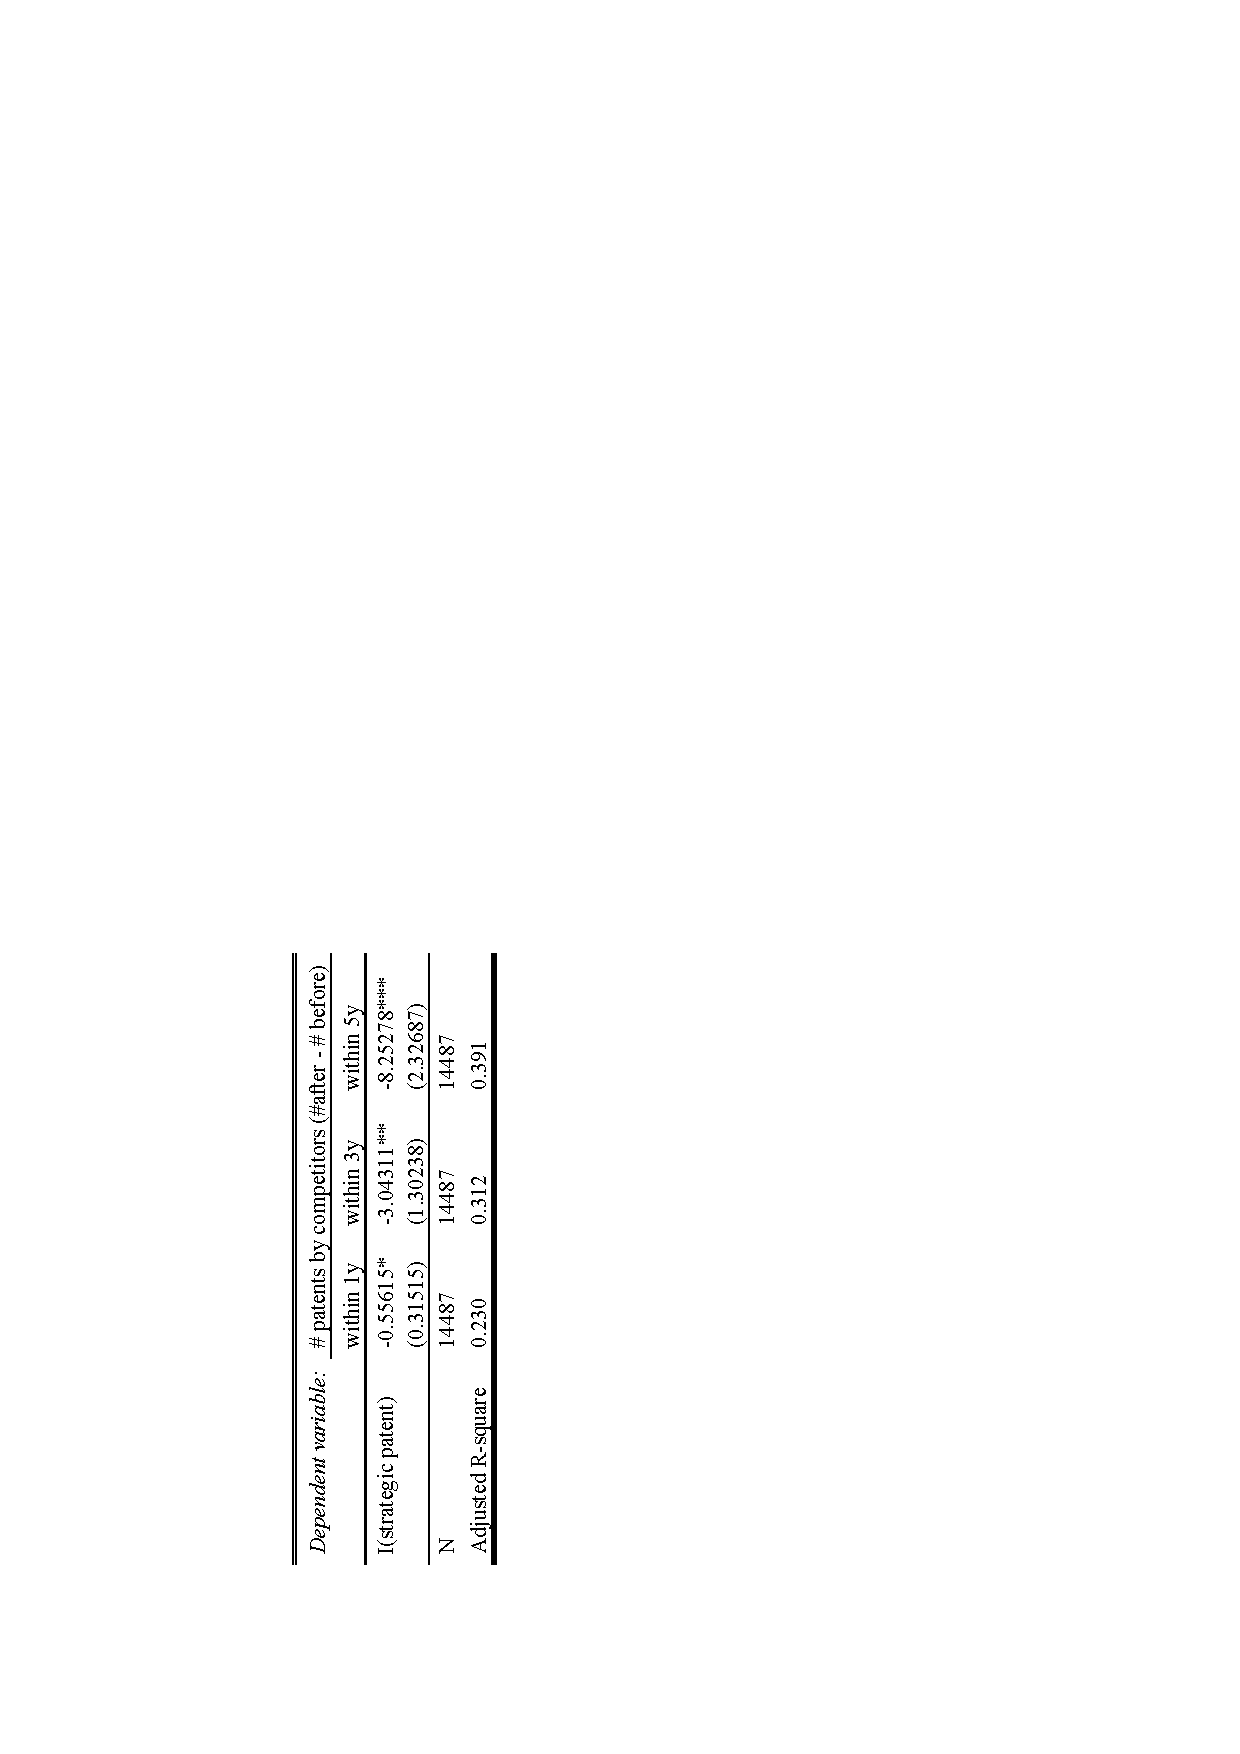
\includegraphics[angle =270,trim = 130 20 40 40, clip]{latex_tables/table_6.pdf}
	}
\end{table}	

\newpage
\begin{landscape}
	\begin{table}[ht!]\centering
		\def\sym#1{\ifmmode^{#1}\else\(^{#1}\)\fi}
		
		\captionsetup{singlelinecheck=off}
		\caption[.]{\textbf{. Strategic Patent Effect on Innovation by Competitors by Market Proximity.} Table reports the results of regression of an indicator of patent strategic status on the change in number of patents filed by the competitors within the same product market defined by TNIC3 by the total average product similarity within the market. The dependent variable is the difference between the total number of patents issued by competitors one, three and five years after and one, three and five years before the filing of the patent by focal firm. The sample is split into firms operating within low (high) product proximity industries, defined as TNIC3 industries with average proximity score measured as in \color{blue}Hoberg, Phillips (2010) \color{black} is below (above) year median. The results are estimated on the sample of top performing patents within the matched sample. Patent applications are classified as top performing if at the date of patent filing the economic value of the patent is higher than the year's median. All specifications control for filing year, examiner art unit and firm fixed effect. Standard errors are clustered at examiner art unit by year of filing. Standard errors are reported in parenthesis. Levels of significance: *10\%, **5\%, and ***1\%.
		}
		\label{tab:stifle_prox}
		\vspace*{0.2in}		
		{\scriptsize
			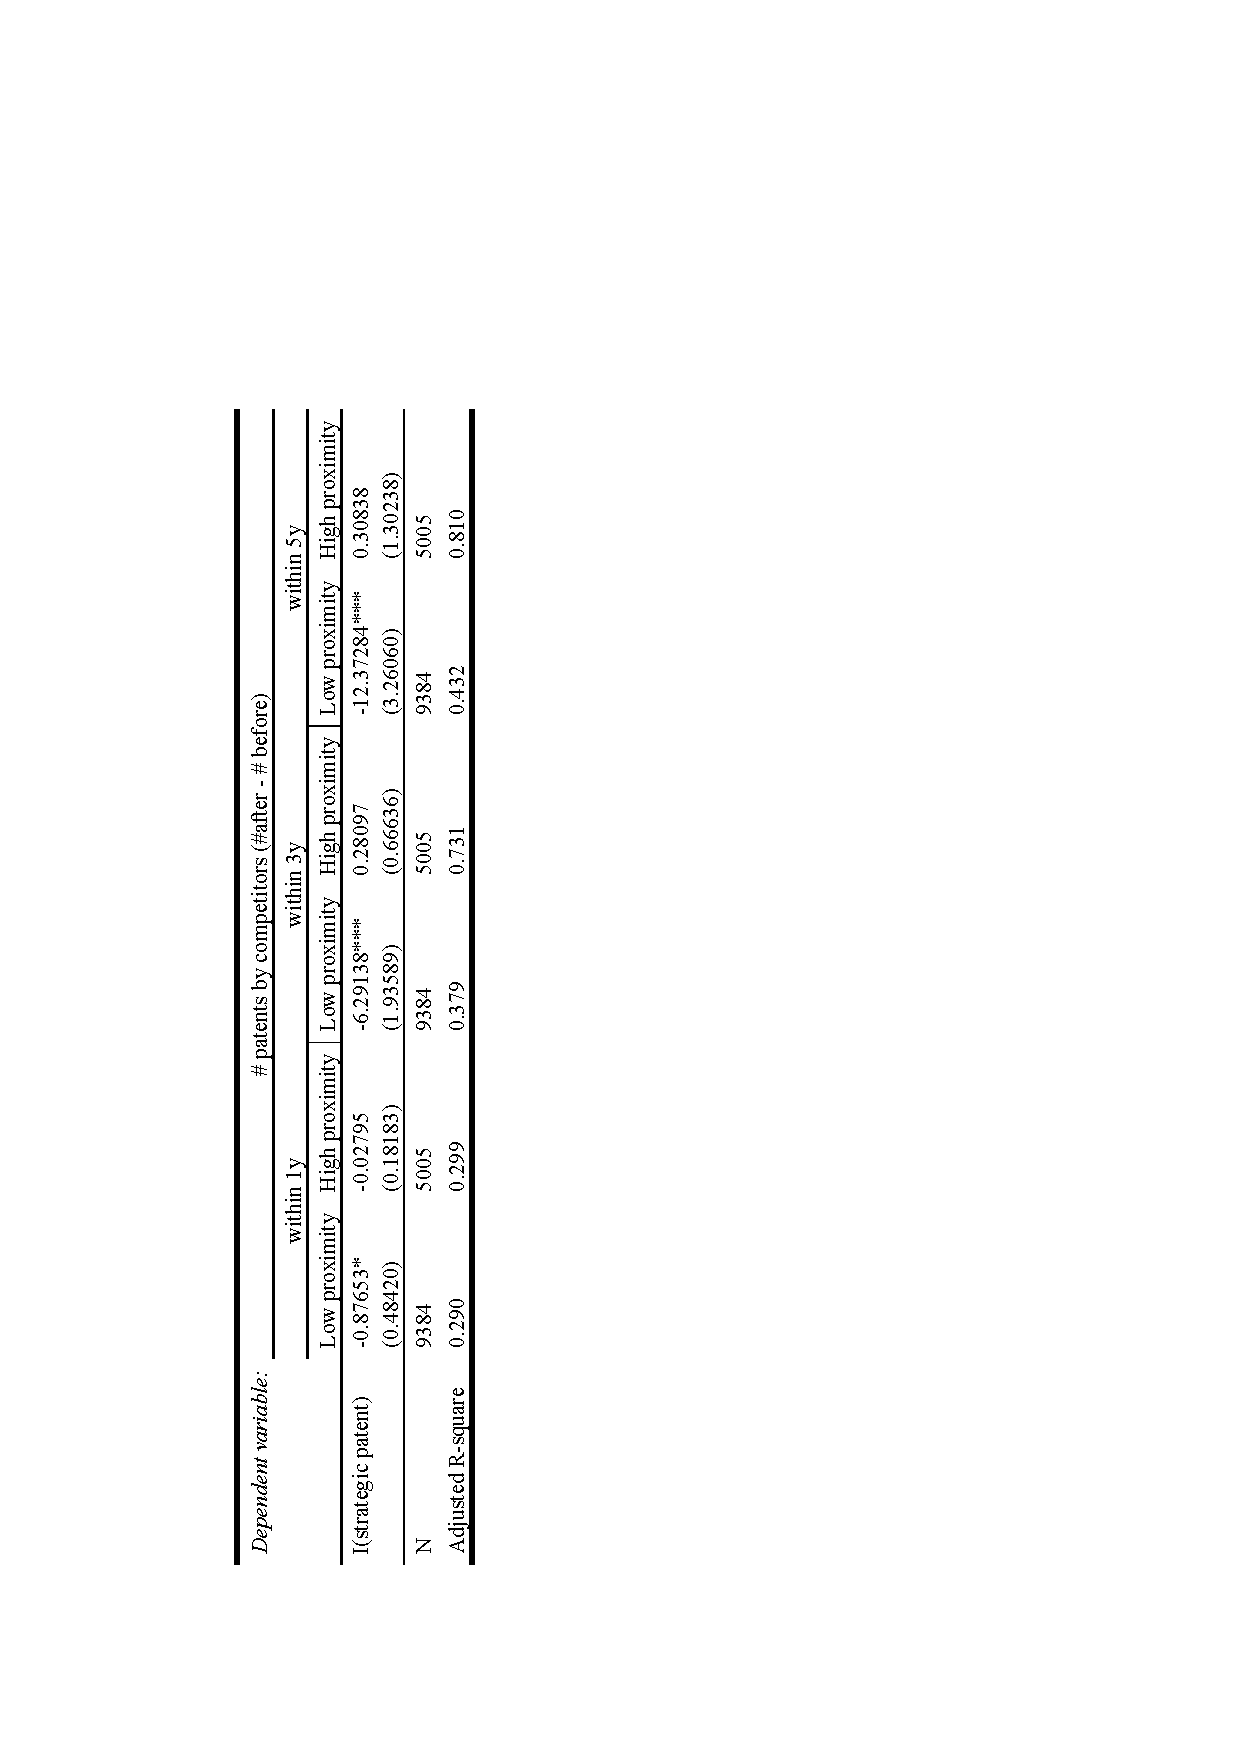
\includegraphics[angle =270,trim = 90 65 40 40, clip]{latex_tables/table_7.pdf}
		}
	\end{table}	
\end{landscape}

\newpage
\begin{table}[ht!]\centering
	\def\sym#1{\ifmmode^{#1}\else\(^{#1}\)\fi}
	
	\captionsetup{singlelinecheck=off}
	\caption[.]{\textbf{. Strategic Patent Effect on Market Concentration and Firm Productivity.} This table shows the results from equation \eqref{eq:reg1} of the impact of strategic patent issue on patentee using the matched sample. The sample is matched exactly on year of patent filing and patent category, and it is matched coarsely on the economic value of the patent and firm's baseline sales outcome (averaged over five pre-filing years). The patent is classified as strategic (productive) if it falls into the top 50\% of the distribution of the private economic value of the patent as measure by eq.\eqref{eq:kogan}, but
		bottom (top) 50\% of distribution of its scientific value (measured by forward citations). Columns (1) and (2) report the effect of productive and a strategic patent grant on post-filing HHI based on TNIC3 industry classification and measured in eq.\eqref{eq:hhi}. Compared to column (1), column (2) adds controls from \autoref{tab:matched_sum}. Columns (3) and (4) repeat the analysis using the number of competitors within the firm's product market as a dependent variable, while columns (5) and (6) report the effect of productive vs strategic patenting on post-filing revenue-based total factor productivity as in \color{blue}Imrohoroglu et al (2013)\color{black}. All specifications control for filing year, examiner art unit and firm fixed effect, as well as baseline measure of the dependent variable (calculated over the five pre-filing years). Standard errors are clustered at examiner art unit by year of filing. Standard errors are reported in parenthesis. Levels of significance: *10\%, **5\%, and ***1\%. 
	}
	\label{tab:result_hhi}
	\vspace*{0.2in}		
	{\scriptsize
		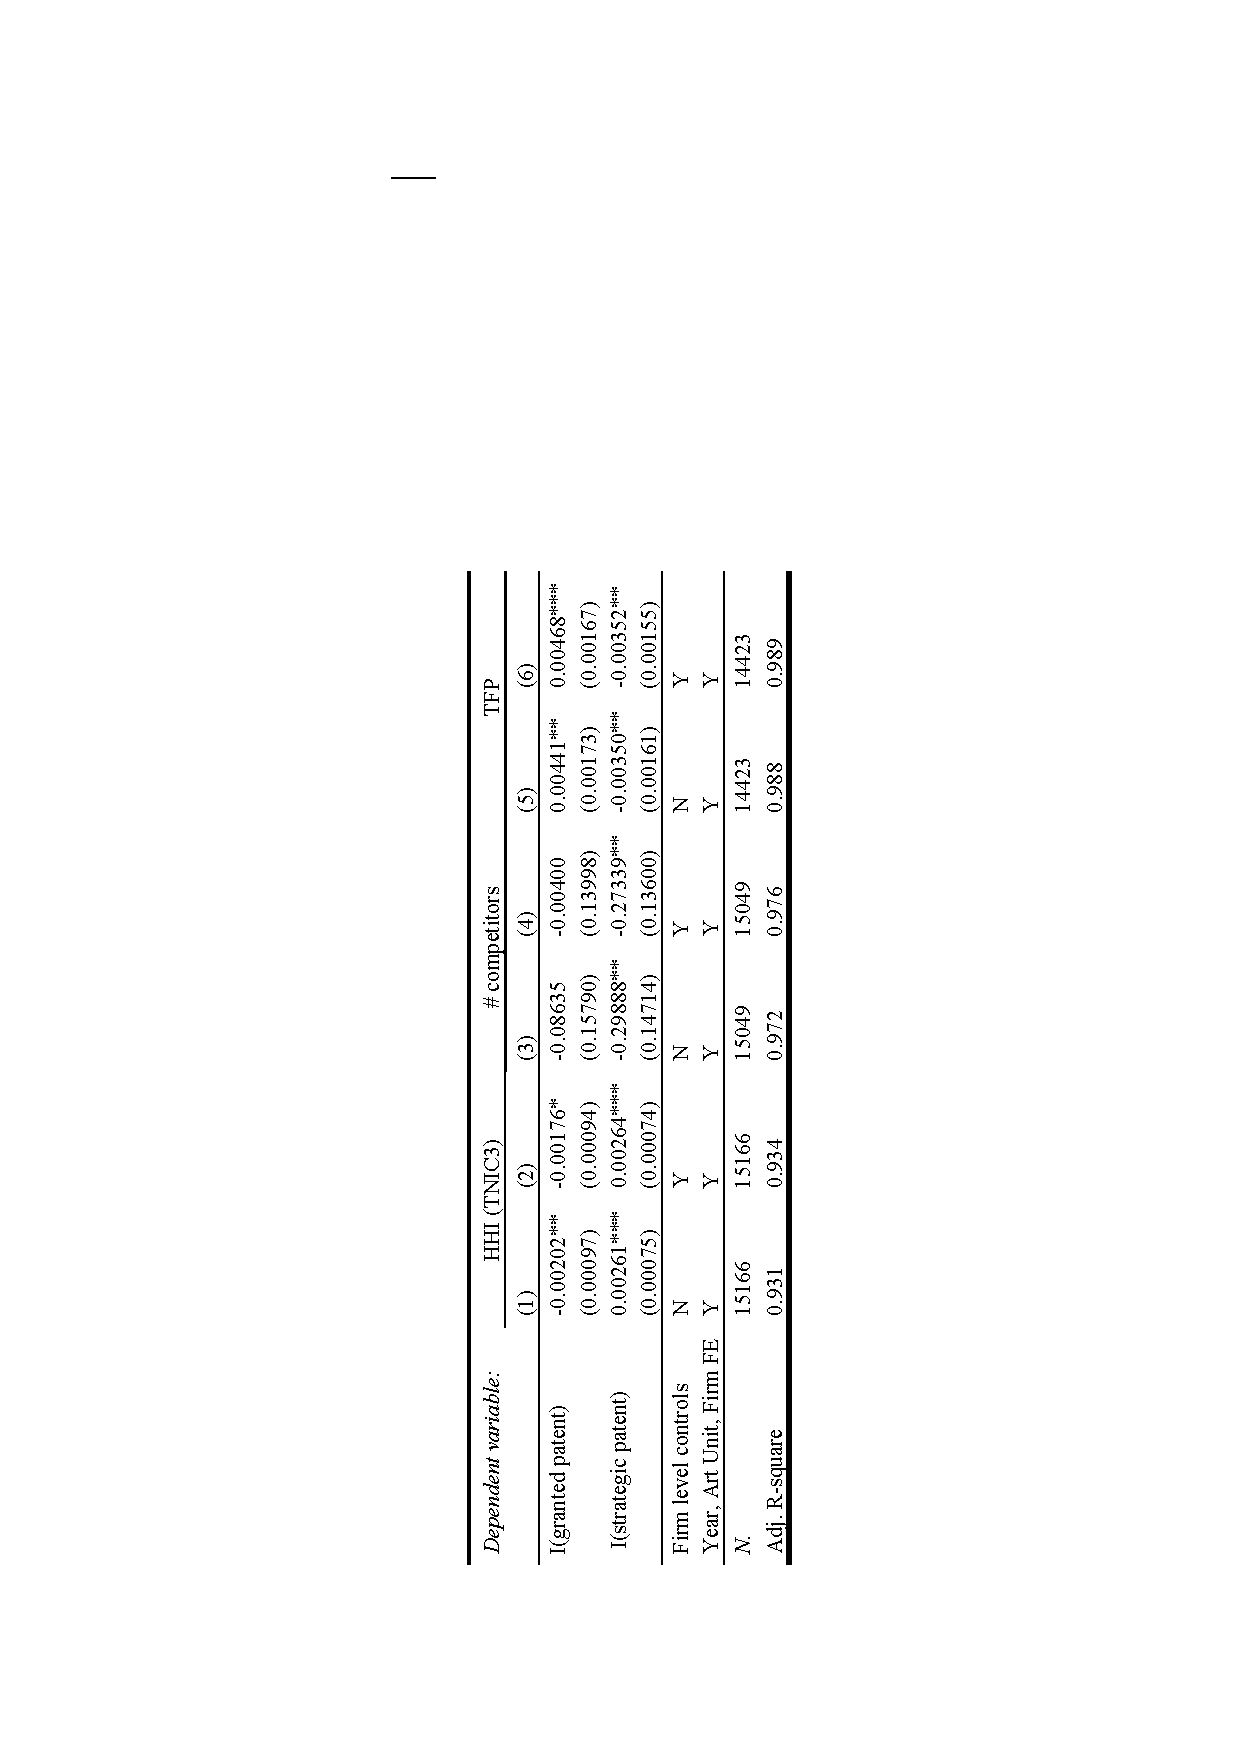
\includegraphics[angle =270,trim = 200 80 40 40, clip]{latex_tables/table_8.pdf}
	}
\end{table}	

\newpage
\begin{table}[ht!]\centering
	\def\sym#1{\ifmmode^{#1}\else\(^{#1}\)\fi}
	
	\captionsetup{singlelinecheck=off}
	\caption[.]{\textbf{. Strategic Patent Effect on Market Concentration by Market Proximity} This table shows the results from equation \eqref{eq:reg1} of the impact of strategic patent issue on patentee using the matched sample separately by group using the total average product similarity within the market. The sample is split into firms operating within low (high) product proximity industries, defined as TNIC3 industries with average proximity score measured as in \color{blue}Hoberg, Phillips (2010) \color{black} is below (above) year median. Columns (1) and (2) report the effect of productive and a strategic patent grant on post-filing HHI based on TNIC3 industry classification and measured in eq.\eqref{eq:hhi}. Columns (3) and (4) repeat the analysis using the number of competitors within the firm's product market as a dependent variable. All specifications control for filing year, examiner art unit and firm fixed effect, as well as firm controls as in \autoref{tab:matched_sum} and baseline measure of the dependent variable (calculated over the five pre-filing years). Standard errors are clustered at examiner art unit by year of filing. Standard errors are reported in parenthesis. Levels of significance: *10\%, **5\%, and ***1\%.
	}
	\label{tab:result_hhi_prox}
	\vspace*{0.2in}		
	{\scriptsize
		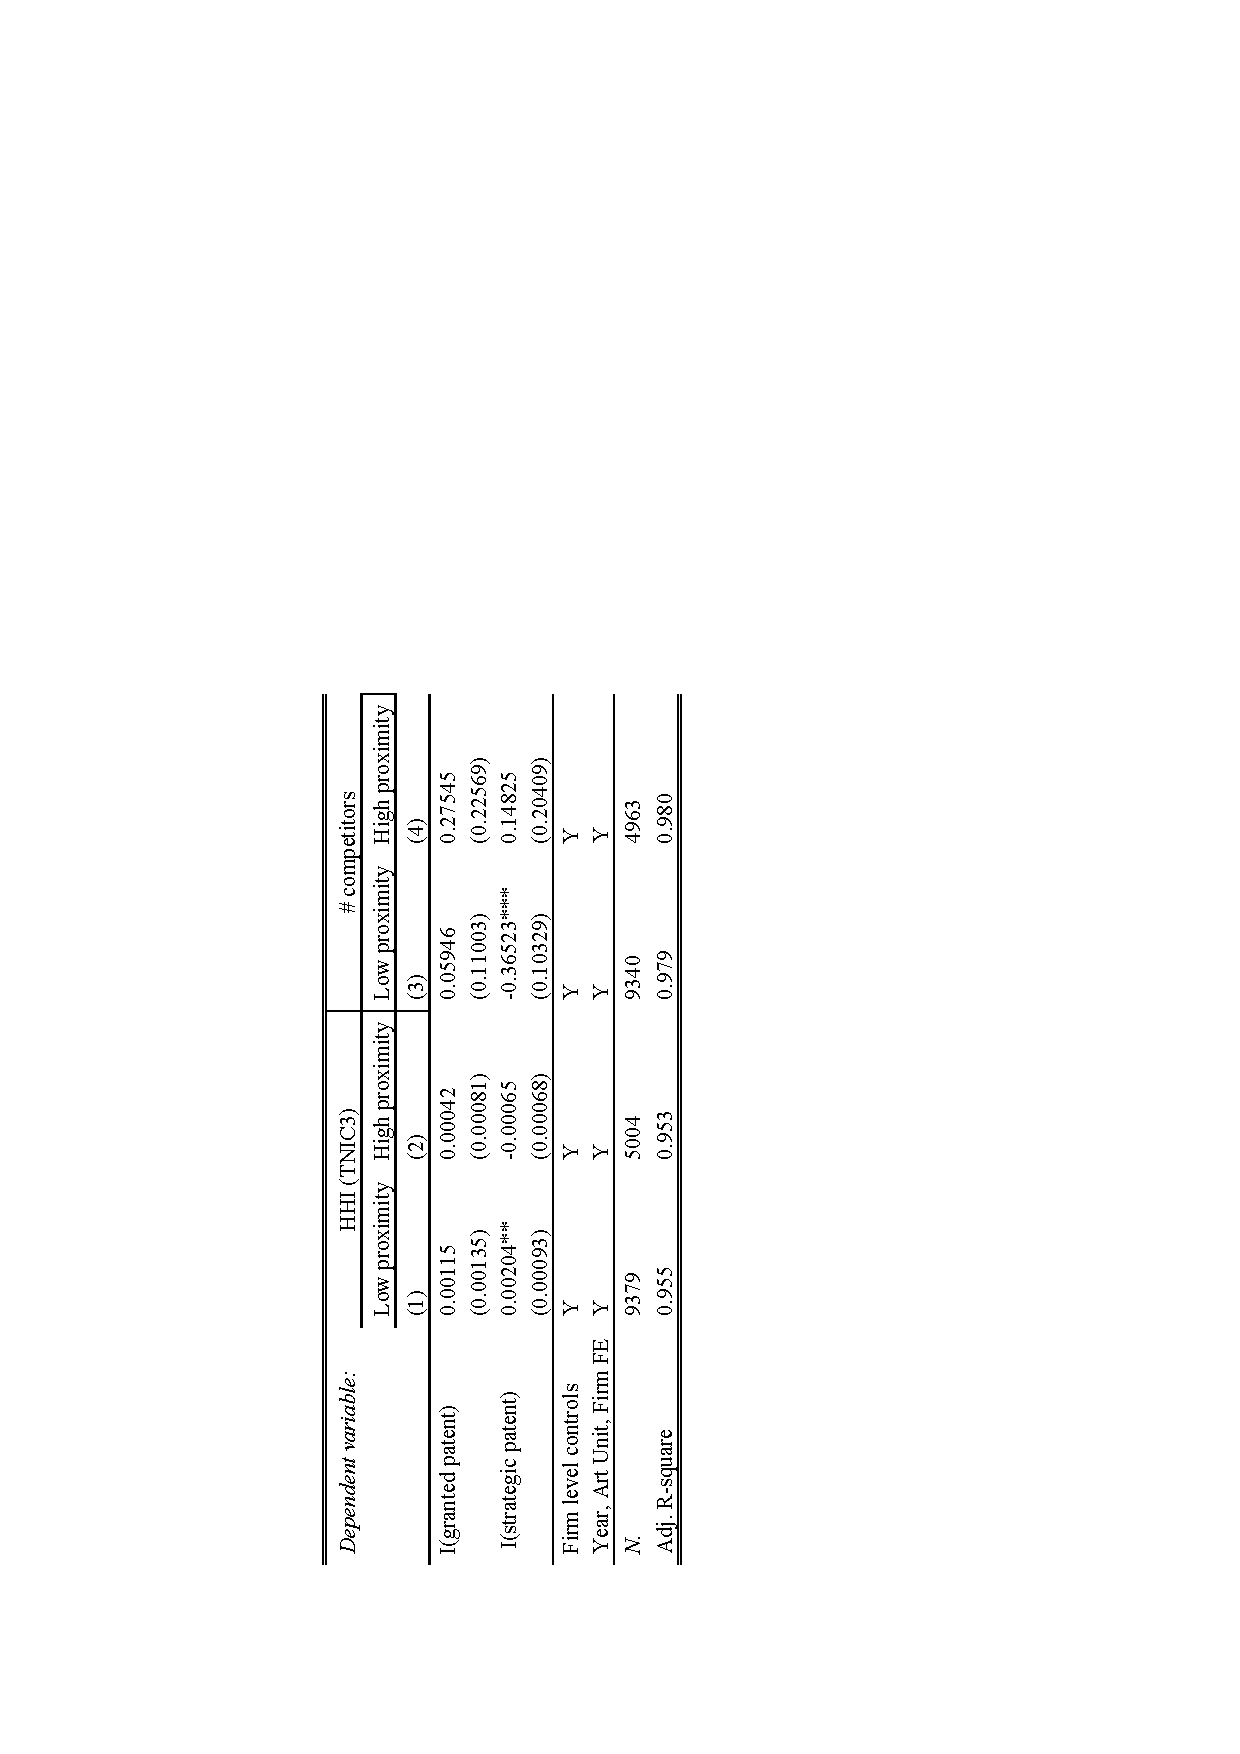
\includegraphics[angle =270,trim = 130 65 40 40, clip]{latex_tables/table_10.pdf}
		
	}
\end{table}	

\newpage
\begin{table}[ht!]\centering
	\def\sym#1{\ifmmode^{#1}\else\(^{#1}\)\fi}
	
	\captionsetup{singlelinecheck=off}
	\caption[.]{\textbf{. Strategic Patent Effect on Market Concentration by Firm's Proximity to Technological Frontier.} This table shows the results from equation \eqref{eq:reg1} of the impact of strategic patent issue on patentee using the matched sample separately by group using the technological proximity of the patentee to the frontier firm. The firm is
		defined as a technological leader if its technological gap measured as in eq.\eqref{eq:gap} is lower than year's median value, signaling that the firm is closer to the frontier firm. If the gap is larger than the year's median value, then
		the firm is classified as a laggard.  Columns (1) and (2) report the effect of productive and a strategic patent grant on post-filing HHI based on TNIC3 industry classification and measured in eq.\eqref{eq:hhi}. Columns (3) and (4) repeat the analysis using the number of competitors within the firm's product market as a dependent variable. All specifications control for filing year, examiner art unit and firm fixed effect, as well as firm controls as in \autoref{tab:matched_sum} and baseline measure of the dependent variable (calculated over the five pre-filing years). Standard errors are clustered at examiner art unit by year of filing. Standard errors are reported in parenthesis. Levels of significance: *10\%, **5\%, and ***1\%.
	}
	\label{tab:result_hhi_prox_gap}
	\vspace*{0.2in}		
	{\scriptsize
		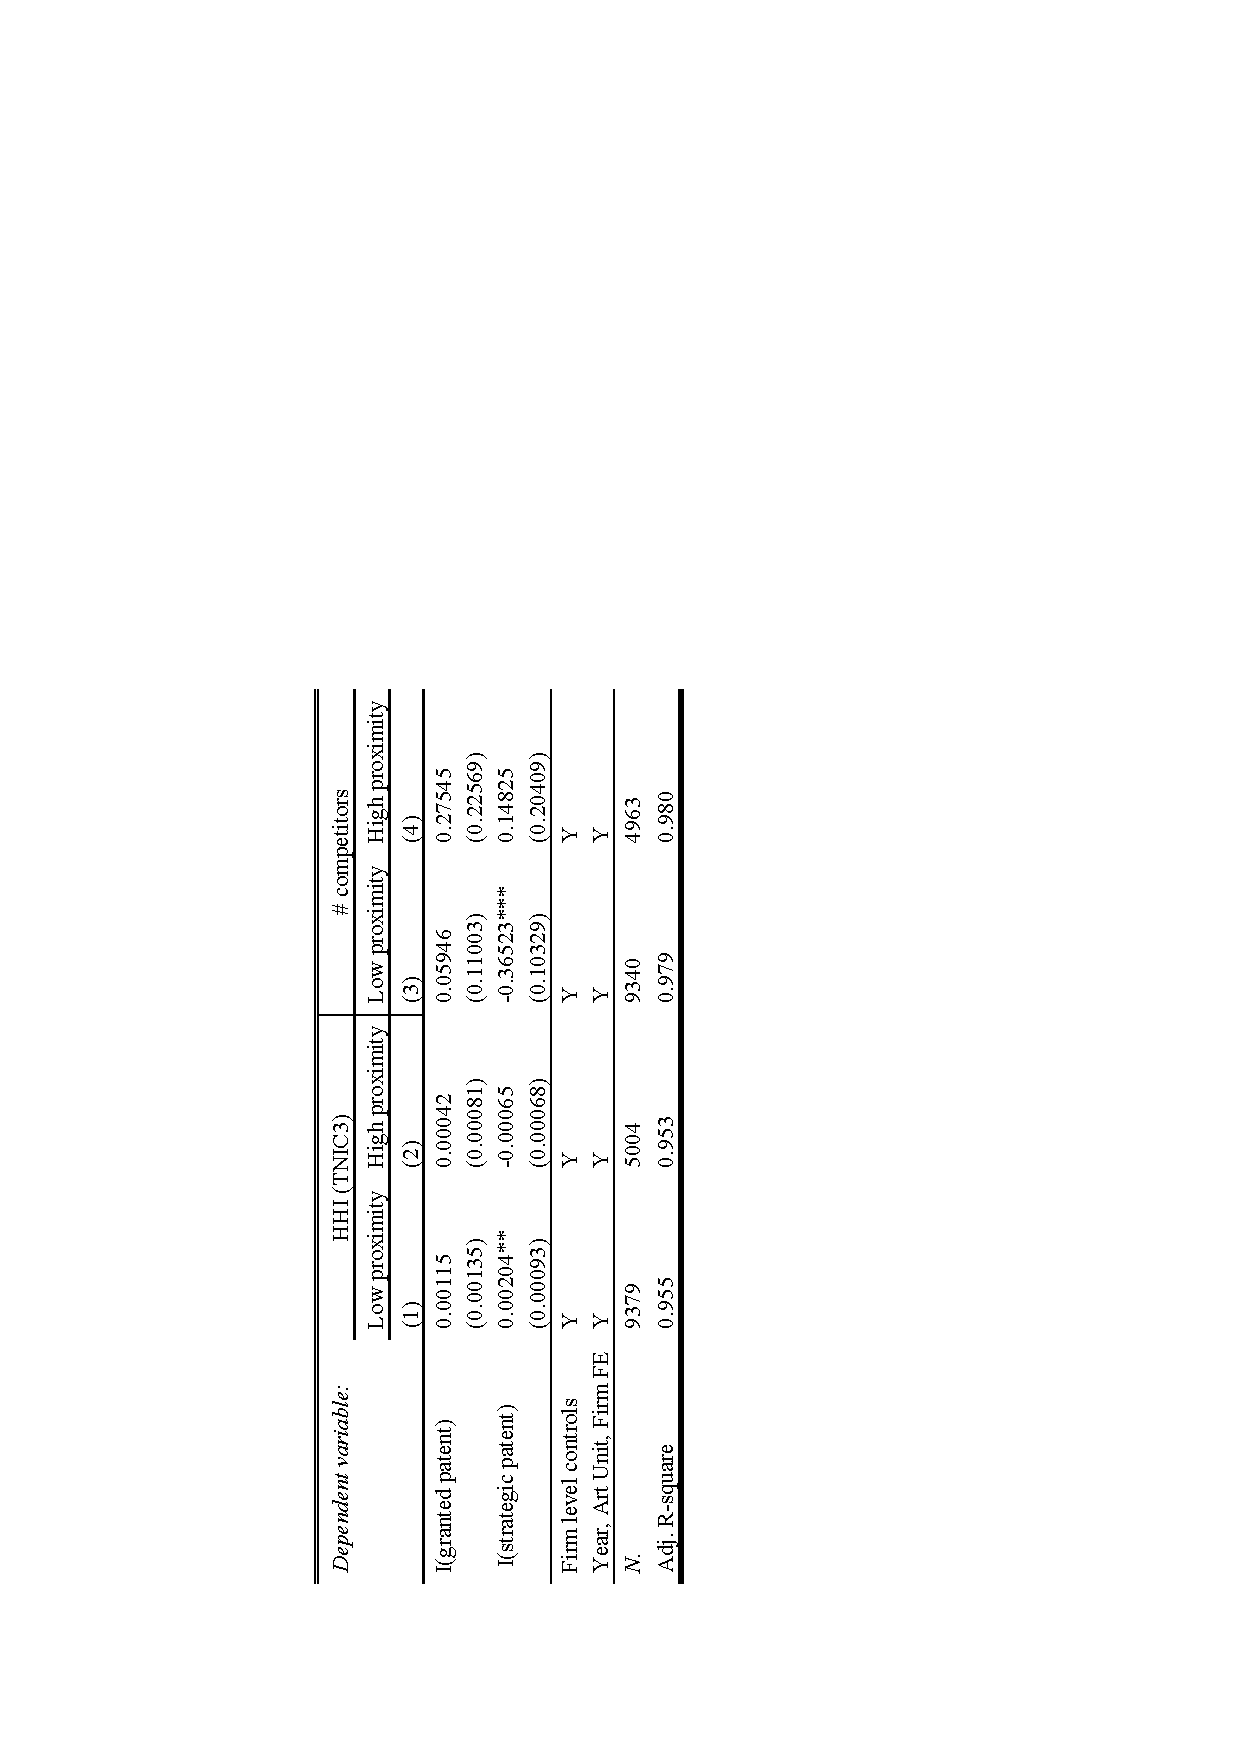
\includegraphics[angle =270,trim = 130 65 40 40, clip]{latex_tables/table_9.pdf}
	}
\end{table}	

\newpage
\begin{table}[ht!]\centering
	\def\sym#1{\ifmmode^{#1}\else\(^{#1}\)\fi}
	
	\captionsetup{singlelinecheck=off}
	\caption[.]{\textbf{. Effect of Strategic Patenting on Future Growth and Productivity: Patenting Firm.} This table reports the estimates of equation \eqref{eq:reg2} for firm profit, sales and TFPR growth over the horizon of one to five years. Profit is measured as a ratio of the sales minus cogs to total assets; TFPR is estimated following  \color{blue}Imrohoroglu et al (2013)\color{black}. All specifications control for filing year, examiner art unit and firm fixed effect, as well as firm controls as in \autoref{tab:matched_sum} and baseline measure of the dependent variable (calculated over the five pre-filing years). Standard errors are clustered at examiner art unit by year of filing. Standard errors are reported in parenthesis. Levels of significance: *10\%, **5\%, and ***1\%.    
	}
	\label{tab:firm_gr}
	\vspace*{0.2in}		
	{\scriptsize
		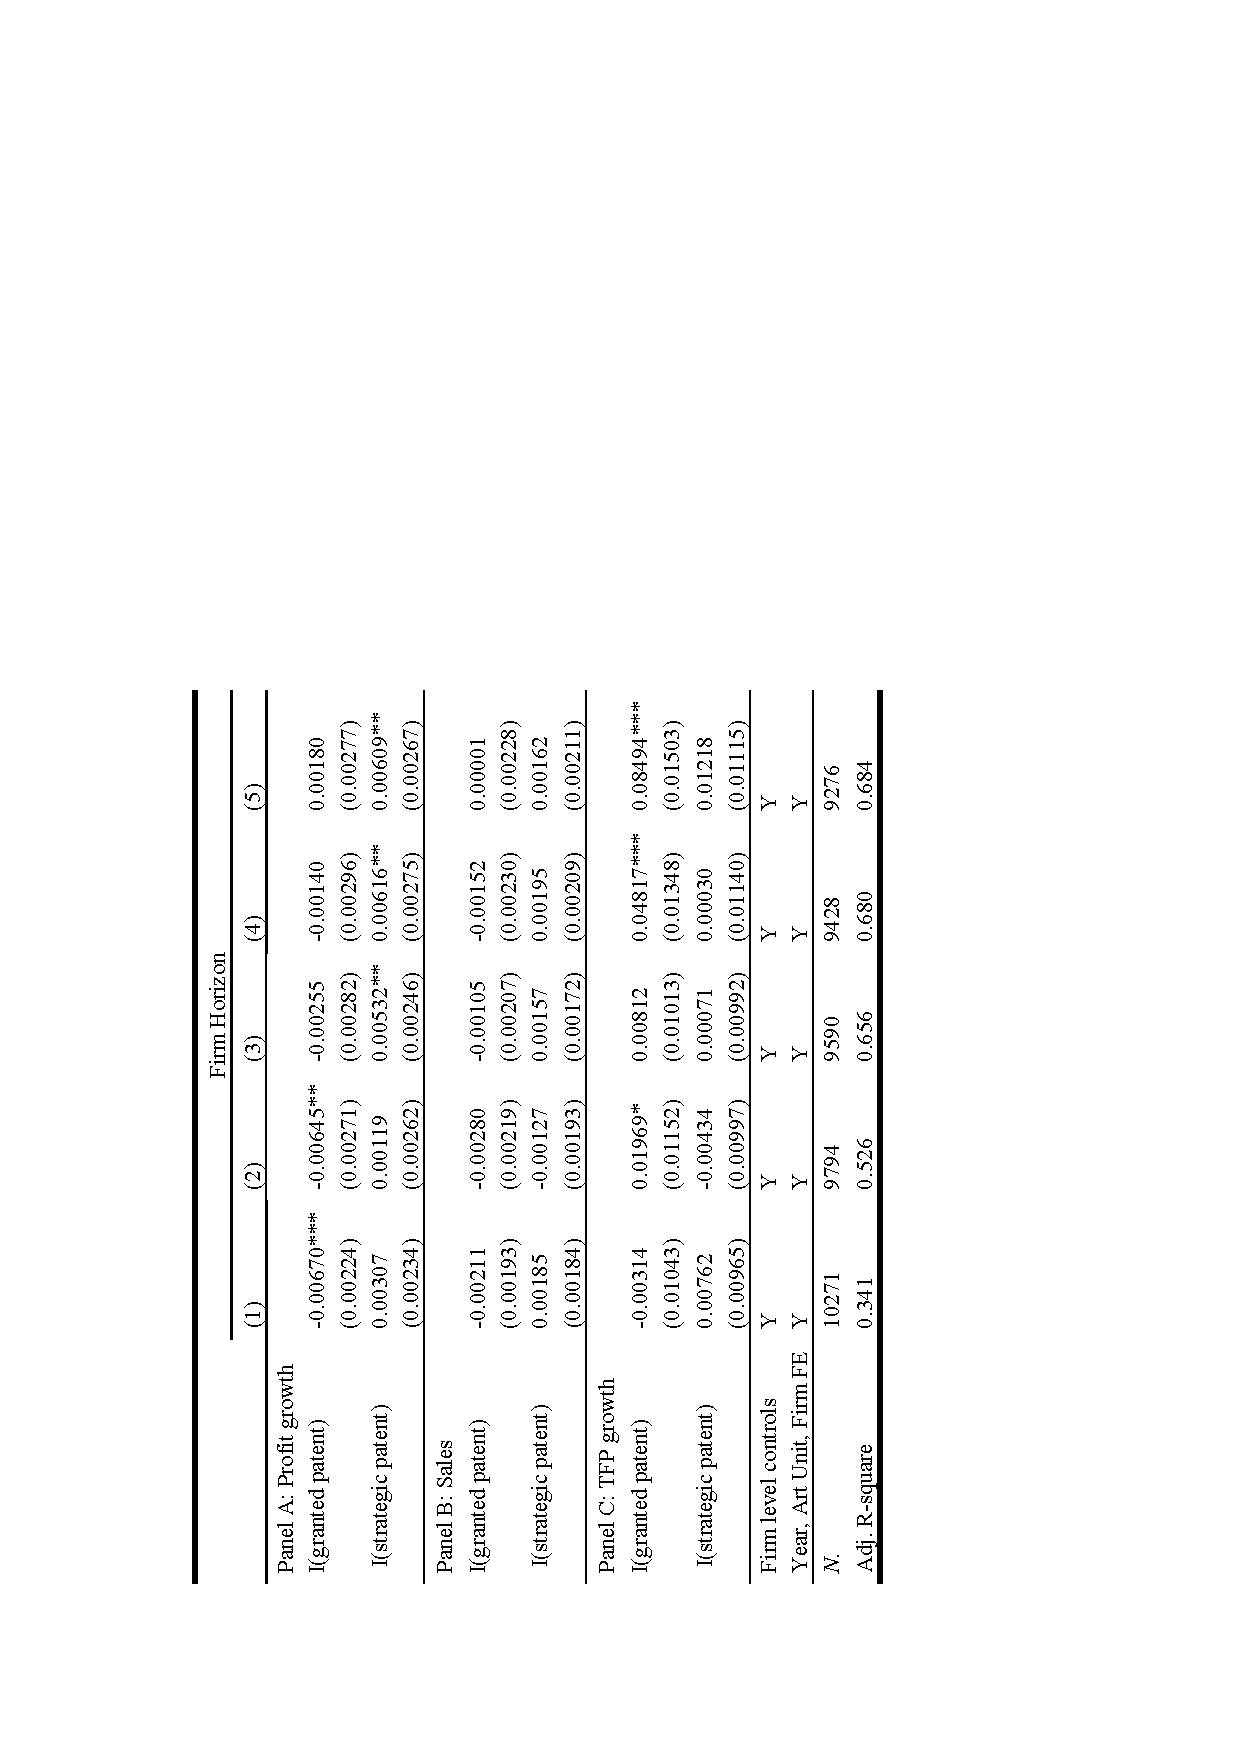
\includegraphics[angle =270,trim = 90 65 40 40, clip]{latex_tables/table_19.pdf}
	}
\end{table}	

\newpage
\begin{table}[ht!]\centering
	\def\sym#1{\ifmmode^{#1}\else\(^{#1}\)\fi}
	
	\captionsetup{singlelinecheck=off}
	\caption[.]{\textbf{. Effect of Strategic Patenting on Future Growth and Productivity: Competitors.} This table reports the estimates of equation \eqref{eq:reg2} for firm profit, sales and TFPR growth over the horizon of one to five years for competitors. Competing firms are defined as top 50th percentile closest peers using TNIC3 industry classification from \color{blue}Hoberg, Phllips (2010)\color{black}. Profit is measured as a ratio of the sales minus cogs to total assets; TFPR is estimated following  \color{blue}Imrohoroglu et al (2013)\color{black}. The dependent variables and controls are calculated as equal-weighted average for specified competing firms. All specifications control for filing year, examiner art unit and firm fixed effect, as well as competitors portfolio controls as in \autoref{tab:matched_sum} and baseline level measures of the dependent variable (calculated over the five pre-filing years). Standard errors are clustered at examiner art unit by year of filing. Standard errors are reported in parenthesis. Levels of significance: *10\%, **5\%, and ***1\%.  
	}
	\label{tab:comp_gr}
	\vspace*{0.2in}		
	{\scriptsize
		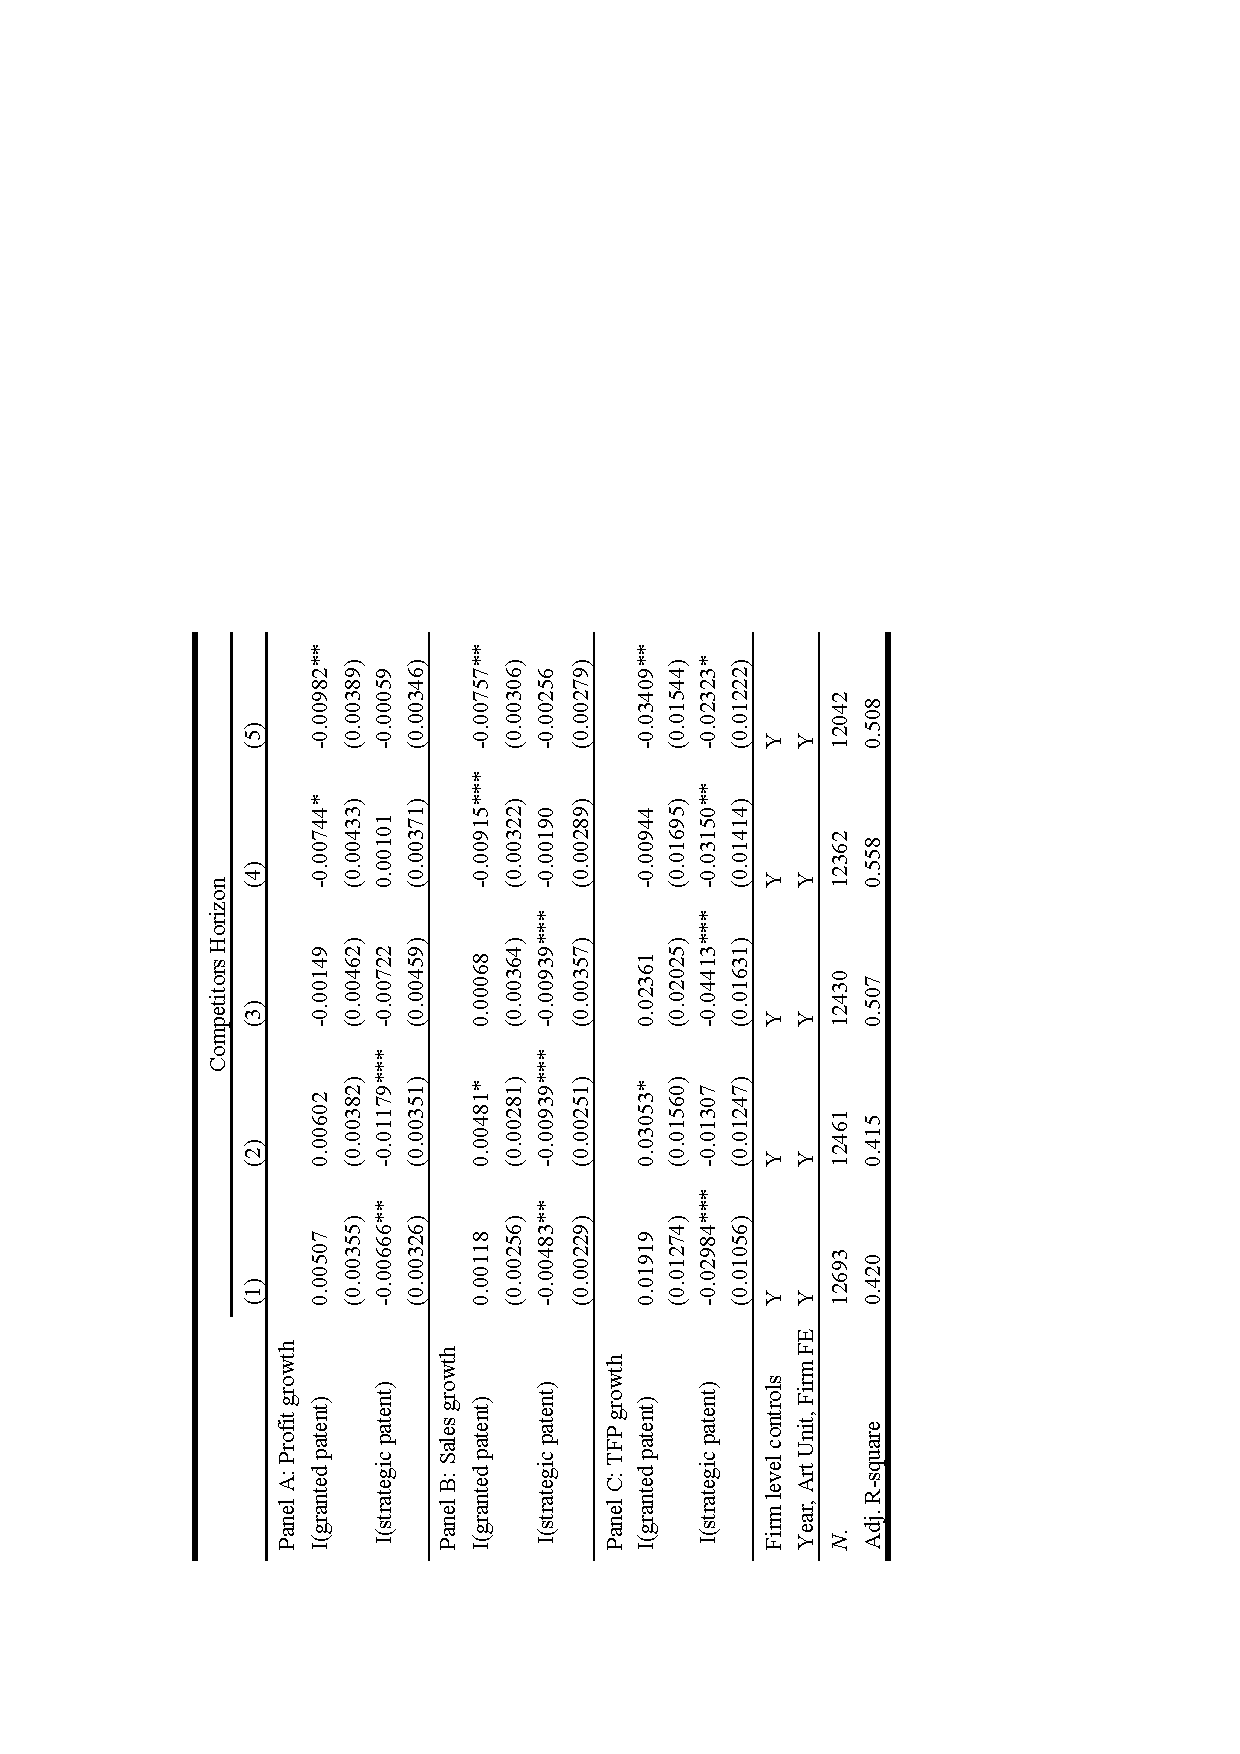
\includegraphics[angle =270,trim = 90 65 40 40, clip]{latex_tables/table_20.pdf}
	}
\end{table}	


\newpage
\begin{landscape}
	
	\begin{table}[ht!]\centering
		\def\sym#1{\ifmmode^{#1}\else\(^{#1}\)\fi}
		
		\captionsetup{singlelinecheck=off}
		\caption[.]{\textbf{. Effect of Strategic Patenting on Future Growth and Productivity by Market and Firm Characteristics.} This table reports the estimates of equation \eqref{eq:reg2} for firm profit, sales and TFPR growth over the horizon of one year for patentee and competitors by product market proximity and patenting firm technological closeness to the frontier. The sample is split into firms operating within low (high) product proximity industries, defined as TNIC3 industries with average proximity score measured as in \color{blue}Hoberg, Phillips (2010) \color{black} is below (above) year median (columns (3) and (4), and (7) and (8)). Columns (1) and (2), and (5) and (6) split the sample of patenting firms into technological leaders if firm's technological gap measured as in eq.\eqref{eq:gap} is lower than year's median value signaling that the firm is closer to the frontier firm, and technological laggards if the gap is larger than the year's median value. Profit is measured as a ratio of the sales minus cogs to total assets; TFPR is estimated following  \color{blue}Imrohoroglu et al (2013)\color{black}.  Competing firms are defined as top 50th percentile closest peers using TNIC3 industry classification. The dependent variables and controls for competitors are calculated as equal-weighted average. All specifications control for filing year, examiner art unit and firm fixed effect, as well as competitors portfolio controls as in \autoref{tab:matched_sum} and baseline level measures of the dependent variable (calculated over the five pre-filing years). Standard errors are clustered at examiner art unit by year of filing. Standard errors are reported in parenthesis. Levels of significance: *10\%, **5\%, and ***1\%. 
		}
		\label{tab:firm_comp_gr}
		\vspace*{0.2in}		
		{\scriptsize
			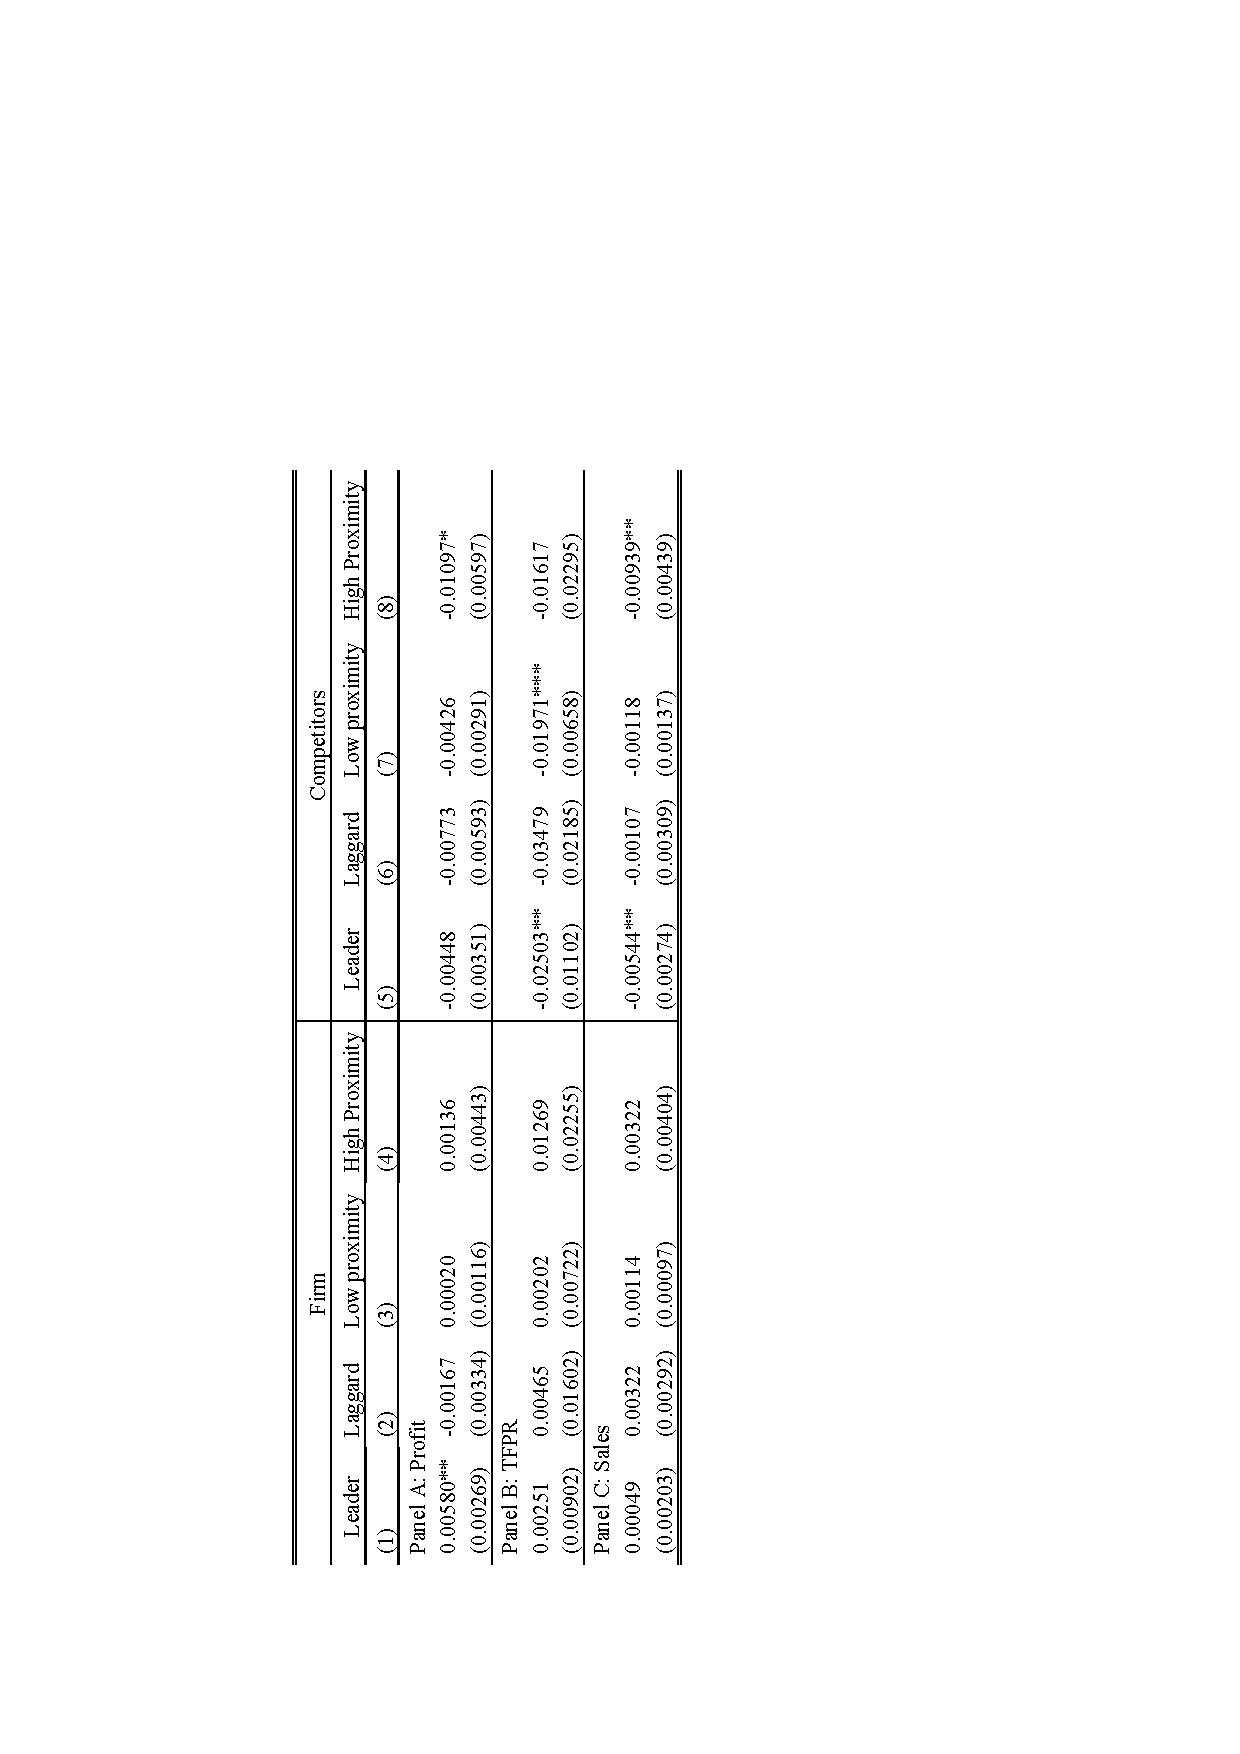
\includegraphics[angle =270,trim = 90 65 40 40, clip]{latex_tables/table_17.pdf}
		}
	\end{table}	
	
\end{landscape}
\newpage



\begin{table}[ht!]\centering
	\def\sym#1{\ifmmode^{#1}\else\(^{#1}\)\fi}
	
	\captionsetup{singlelinecheck=off}
	\caption[.]{\textbf{. Robustness: Effect of Strategic Patenting on Future Growth and Productivity.} This table reports the estimates of equation \eqref{eq:reg2} for firm profit, sales and TFPR growth over the horizon of one year for patentee and competitors controlling for competitors' innovative activity. Patenting by competitors is estimated using the total number of patents filed by the peers within TNIC3 industry one year before and one year after the patent application by the focal firm. Profit is measured as a ratio of the sales minus cogs to total assets; TFPR is estimated following  \color{blue}Imrohoroglu et al (2013)\color{black}.  Competing firms are defined as top 50th percentile closest peers using TNIC3 industry classification. The dependent variables and controls for competitors are calculated as equal-weighted average. All specifications control for filing year, examiner art unit and firm fixed effect, as well as competitors portfolio controls as in \autoref{tab:matched_sum} and baseline level measures of the dependent variable (calculated over the five pre-filing years). Standard errors are clustered at examiner art unit by year of filing. Standard errors are reported in parenthesis. Levels of significance: *10\%, **5\%, and ***1\%. 
	}
	\label{tab:robust_p}
	\vspace*{0.2in}		
	{\scriptsize
		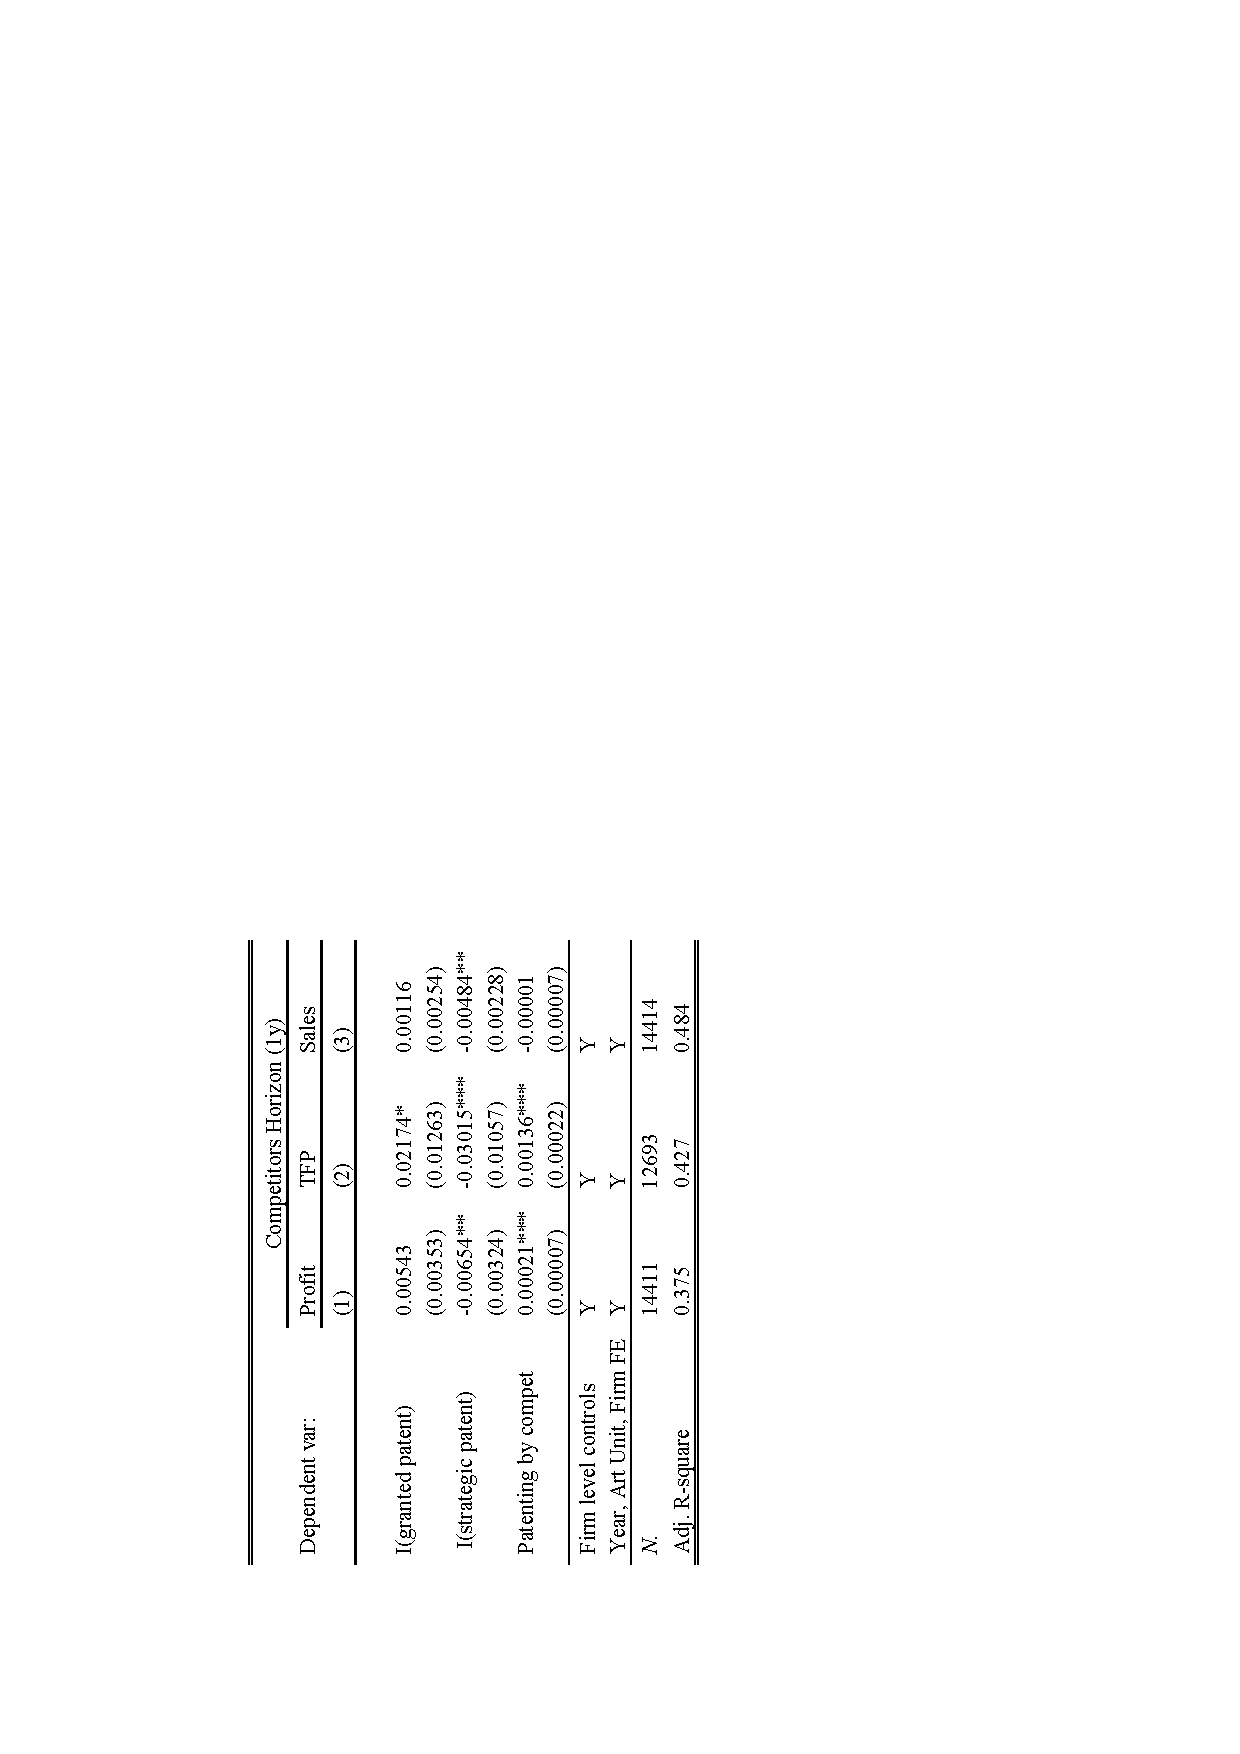
\includegraphics[angle =270,trim = 90 20 40 40, clip]{latex_tables/table_18.pdf}
	}
\end{table}	



\end{document}